\documentclass[oneside, 12pt]{book}

\usepackage[utf8]{inputenc}
\usepackage[a4paper, top=3cm, bottom=3cm, left=2cm, right=2cm]{geometry}
\usepackage{amsmath}
\usepackage{graphicx}
\usepackage[dvipsnames]{xcolor}
\usepackage[hidelinks]{hyperref}
\usepackage{csvsimple}
\usepackage{booktabs}
\usepackage{siunitx}
\usepackage{setspace}
\usepackage{amsthm}
\usepackage{float}
\usepackage{tikz}
\usepackage[toc,page]{appendix}
\usepackage{minted}
\usepackage{caption}
\usepackage{subcaption}
\usepackage{pdfpages}
\RecustomVerbatimEnvironment{Verbatim}{BVerbatim}{}
\usetikzlibrary{shapes.multipart}
\usetikzlibrary{positioning}
\usetikzlibrary{decorations.pathreplacing}
\makeatletter
\AtBeginEnvironment{minted}{\dontdofcolorbox}
\def\dontdofcolorbox{\renewcommand\fcolorbox[4][]{##4}}
\makeatother

\setlength{\parindent}{0pt}
\setlength{\parskip}{1em}
\setstretch{1.25}
\hyphenation{Prolog}
\hyphenation{WebAssembly}
\theoremstyle{definition}
\newtheorem*{definition}{Definition}

\begin{document}

\newgeometry{top=1in, bottom=1in, left=1in, right=1in}
\begin{titlepage}

\setlength{\baselineskip}{2em}

\centering

\begin{minipage}{0.5\textwidth}
  
\includegraphics[width=5cm]{_cambridge.png}
\end{minipage}%
\begin{minipage}[t]{0.5\textwidth}
  \hfill \Large \scshape William Henderson
\end{minipage}

\vspace*{65mm}

{\Huge \bf A Prolog interpreter \\
for the browser}

\vspace*{10mm}

{\Large Churchill College \\
\Large University of Cambridge}

\vspace*{10mm}

{\Large May 2025}

\vspace*{65mm}

{\large Submitted as part of the requirements for} \\
{\large \it Part II of the Computer Science Tripos}

\end{titlepage}
\restoregeometry

\frontmatter

\chapter*{Declaration}

I, the candidate for Part II of the Computer Science Tripos with Blind Grading Number 2384E, hereby declare that this report and the work described in it are my own work, unaided except as may be specified below, and that the report does not contain material that has already been used to any substantial extent for a comparable purpose. In preparation of this report, I adhered to the Department of Computer Science and Technology AI Policy. I am content for my report to be made available to the students and staff of the University.

Signed {\it William Henderson} \\
Date {\it \today}

\hfill {
  \begin{tabular}{c}
    
\includegraphics[width=0.3\textwidth]{signature.png} \\
    \hline \rule{0pt}{1.2em} William Henderson
  \end{tabular}
}

\chapter*{Proforma}

{\large \begin{tabular}{ll}
Candidate Number: & {\bf TBD} \\
Project Title: & {\bf A Prolog interpreter for the browser} \\
Examination: & {\bf Computer Science Tripos -- Part II, 2025} \\
Word Count: & {\bf TBD} \\
Code Line Count: & {\bf TBD} \\
Project Originator: & {\bf The candidate} \\
Supervisor: & {\bf Prof. Alan Mycroft}
\end{tabular}}

\section*{Original Aims of the Project}

TODO

\section*{Work Completed}

TODO 

\section*{Special Difficulties}

None.

\tableofcontents

\mainmatter

\chapter{Introduction}

This dissertation explores the use of Prolog in the browser by building a Prolog interpreter, WebPL, that runs in the browser using WebAssembly. This chapter introduces the motivation for the project, briefly discussing the existing landscape of Prolog implementations for the browser, and outlines the aims of the project.

\section{Motivation}

Web pioneer Marc Andreessen claimed in the early days of the Web that ``the browser will be the operating system'': the browser would become the platform on which modern applications are built \cite{kosnerAlwaysEarlyMarc2012}. With increasingly sophisticated applications being delivered through the browser, this vision is proving more and more correct. In the last decade, the development of WebAssembly, a low-level binary instruction format for the Web, has further bridged the gap between browser-based and native applications, enabling web applications to run with near-native performance \cite{haasBringingwebspeed2017}.

The Prolog logic programming language is not exempt from this trend. Prolog is used on the Web in a variety of applications, including for browser-based development environments like SWISH \cite{wielemakerSWISHSWIPrologSharing2015}, enforcing dependency constraints in JavaScript packages\footnote{\url{https://v3.yarnpkg.com/features/constraints}}, and as a query language for databases \cite{wielemakerUsingPrologFundament2007}.

Traditional Prolog Web applications typically use a client-server architecture. The aforementioned Prolog development environment SWISH is one such application: SWI-Prolog runs on the server, communicating with the browser using Pengines, a library for exchanging Prolog queries and results over HTTP \cite{lagerPenginesWebLogic2014}. There are several drawbacks of this model. A dedicated server is required to run the Prolog engine, which may be costly, and latency is introduced by the need for network communication. Running the Prolog engine in the browser directly would eliminate these drawbacks; indeed, Flach concludes that ``an in-browser solution is probably the future of Prolog on the web'' \cite{flachSimplyLogicalFirst2023}.

There are several Prolog implementations that run in the browser, which fall into two categories: general-purpose native implementations that have been ported to WebAssembly, which I will call \emph{web-ported} implementations, and implementations that have been designed from the ground up specifically for the Web, which I will call \emph{web-native} implementations. The former category includes SWI-Prolog \cite{wielemakerSWIProlog2012} and Trealla Prolog \cite{davisonTreallaProlog2020}, while a notable example of the latter is Tau Prolog \cite{riazaTauPrologProlog2024}, written in JavaScript. At the time of writing, there are no web-native implementations that use WebAssembly.

Web-ported implementations enjoy WebAssembly's near-native performance but suffer from poor integration with the browser environment and large binary sizes. The resource requirements of applications in the browser differ greatly from those of native applications, particularly in terms of memory, and web-ported implementations are typically heavyweight and do not take this into account.

Web-native implementations, on the other hand, are more tightly integrated with the browser environment, but are yet to gain the performance benefits of WebAssembly. Furthermore, JavaScript's memory management is entirely independent of the Prolog engine, so information about the state of the Prolog engine cannot be used to optimise allocation and deallocation of memory.

I hypothesise that \textbf{a web-native Prolog implementation using WebAssembly, with design guided by the constraints of the browser environment, may be able to achieve superior performance compared to existing implementations, while preserving tight integration with the browser}. The project explores this hypothesis by building such a Prolog implementation.

\section{Project Aims}

The aims of the project are as follows:

\begin{itemize}
\item to \textbf{build a web-native Prolog implementation} that uses WebAssembly, with a particular focus on performance and browser integration, including
\begin{itemize}
\item a \textbf{lexer} and \textbf{parser} for \emph{pure Prolog}\footnote{So as not to distract from the focus of performance and browser integration, the project considers a subset of Prolog, roughly equivalent to the content of the Cambridge Computer Science Part IB Prolog course. Appendix \ref{appendix:pure-prolog} comprises a detailed definition of the subset.} programs, and
\item an \textbf{interpreter} for the parsed programs,
\end{itemize}
\item to \textbf{make optimisations} to improve performance, including both traditional Prolog optimisations and those that specifically target the browser environment, and
\item to \textbf{evaluate its performance}, both in terms of execution time and memory usage, against existing web-ported and web-native Prolog implementations, exploring which factors contribute to the performance differences.
\end{itemize}

As extensions, the project has the following additional aims:

\begin{itemize}
\item to \textbf{build a browser-based development environment} for the Prolog implementation, similar to SWISH, which supports \textbf{plugins} for other Prolog implementations to facilitate comparison,
\item to \textbf{implement a garbage collector} to make more efficient use of memory, and
\item to \textbf{develop a foreign function interface}, extending the Prolog syntax to support \textbf{inline JavaScript code}, to integrate with the browser environment.
\end{itemize}

\chapter{Preparation}

This chapter introduces Prolog (Section \ref{sec:prolog}) and how garbage collection techniques can be applied to it (Section \ref{sec:prolog-gc}). It also discusses web development with WebAssembly (Section \ref{sec:webdev}), before describing the tools (Section \ref{sec:tools}) and development methodology (Section \ref{sec:dev-methodology}) used in the implementation of the Prolog interpreter. Finally, a requirements analysis is performed (Section \ref{sec:requirements}) and the starting point of the project stated (Section \ref{sec:starting-point}).

\section{Prolog}

\label{sec:prolog}

Prolog is rooted in the fundamental idea that logic can be used as a programming language \cite{kowalskiPredicateLogicProgramming1974}. This section summarises the theory behind Prolog, as well as its execution model and practical implementation details.

\subsection{Clauses and Terms}

Prolog is based on \emph{first-order logic}, specifically \emph{Horn clauses}, which are of the form
$$
B \leftarrow A_1 \land \cdots \land A_n
$$
where $B$ is a positive literal (the \emph{head}) and $A_1, \ldots, A_n$ are negative literals (the \emph{body}). The key insight of Kowalski's \emph{logic programming} paradigm is that we can interpret Horn clauses as procedures of a simple programming language, written in Prolog syntax as
$$
\texttt{B :- A$_1$, $\ldots$, A$_n$.}
$$
A \emph{fact} is a Horn clause with an empty body, and a \emph{goal} is a Horn clause with an empty head.
$$
\texttt{B.} \quad \text{(fact)} \qquad\qquad\qquad \texttt{?- A$_1$, $\ldots$, A$_n$.} \quad \text{(goal)}
$$

Prolog clauses are built up from \emph{terms}, which may be
\begin{itemize}
\item \emph{atoms}, which are either \emph{constants} (e.g. \texttt{a}, \texttt{42}, \texttt{foo}) or \emph{variables} (e.g. \texttt{X}, \texttt{Var}), or
\item \emph{compound terms}, which consist of a \emph{functor} (an atom) and a list of \emph{arguments}, which are terms themselves (e.g. \texttt{is\_even(X)}, \texttt{city(cambridge, united\_kingdom)}).
\end{itemize}

A Prolog program comprises a set of clauses, along with a \emph{query}, which is a goal clause. The aim of the Prolog execution is to find a \emph{substitution} (an assignment of terms to variables) that makes the query true with respect to the program.

\subsection{Most General Unification}

\emph{Unification} is the process of finding a \emph{substitution} that makes two terms equal. A substitution $\theta$ is a set of variable assignments, written $[t_1/x_1, \ldots, t_n/x_n]$, where $t_i$ are terms and $x_i$ distinct variables. A substitution is a \emph{unifier} of two terms $t_1$ and $t_2$ if $t_1\theta = t_2\theta$. The \emph{most general unifier} (MGU) $\theta$ of two terms is a unifier that is more general than any other unifier, that is, all other unifiers $\phi$ can be written as the composition of $\theta$ and another substitution $\psi$. This ensures that, if a solution exists, it will not be missed.

\paragraph{Martelli-Montanari Algorithm}

The \emph{Martelli-Montanari algorithm} is an algorithm for computing the most general unifier of two terms $t_1$ and $t_2$ \cite{martelliEfficientUnificationAlgorithm1982}. It iteratively applies rules to a set of equations, starting with $\{t_1 = t_2\}$, until no more rules can be applied, at which point the remaining set of equations is the unifier.

The rules are shown in Figure \ref{fig:martelli-montanari}. $s$ and $t$ are terms, $X$ and $Y$ are variables, $f$ and $g$ are function symbols, and $S$ is a set of equations. $\text{vars}(t)$ denotes the set of variables occurring in $t$.

\begin{figure}[H]
\begin{align*}
\{f(s_1, \ldots, s_n) = f(t_1, \ldots, t_n)\} \cup S &\rightarrow \{s_1 = t_1, \ldots, s_n = t_n\} \cup S \\
\{f(s_1, \ldots, s_n) = g(t_1, \ldots, t_m)\} \cup S &\rightarrow \text{fail} \\
\{X = X\} \cup S &\rightarrow S \\
\{X = t\} \cup S &\rightarrow \{X = t\} \cup S[t/X] \quad \text{if } X \notin \text{vars}(t) \\
\{X = t\} \cup S &\rightarrow \text{fail} \quad \text{if } X \in \text{vars}(t) \land X \neq t
\end{align*}
\caption{The Martelli-Montanari algorithm}
\label{fig:martelli-montanari}
\end{figure}

The condition $X \notin \text{vars}(t)$ is called the \emph{occurs check}, and is included to prevent the creation of infinite terms. In Prolog, the occurs check is often disabled by default for performance reasons, which enables the representation of cyclic terms.

\subsection{Resolution}

\emph{Resolution} enables the inference of new clauses from existing clauses. In particular, the more restrictive \emph{SLD resolution} (selective linear definite resolution) is the basis of Prolog's execution model.

Given a goal clause \texttt{?- A$_1$, $\ldots$, A$_n$}, and a definite clause \texttt{C :- B$_1$, $\ldots$, B$_m$}, such that $C$ and some $A_i$ unify with MGU $\theta$, a new goal clause can be derived by applying the resolution rule:
$$
\frac{\texttt{C :- B$_1$, $\ldots$, B$_m$} \qquad \texttt{?- A$_1$, $\ldots$, A$_n$}}{(\texttt{?- A$_1$, $\ldots$, A$_{i-1}$, A$_{i+1}$, $\ldots$, A$_n$, B$_1$, $\ldots$, B$_m$})\theta}
$$

\subsection{Execution Model}

Given a Prolog program consisting of a set of clauses and a query, Prolog aims to find a substitution that makes the query true by negating the query and searching for a substitution that refutes the negated query, that is, for which the disjunction of the clauses and the negated query is false. SLD resolution implicitly constructs a \emph{search tree} of possible substitutions, and the execution model of Prolog can be understood as a depth-first search of this tree. Consider the following Prolog program.

\begin{center}
\begin{minted}{prolog}
king(united_kingdom, charles).
king(denmark, frederik).
country(united_kingdom).
country(france).
country(denmark).

?- country(C), king(C, K).
\end{minted}
\end{center}

The execution of this program explores the search tree shown in Figure \ref{fig:prolog-search-tree}.

\begin{figure}[H]
\begin{center}
  \begin{tikzpicture}
      \node (A) at (0,3) {\mintinline{prolog}{country(C), king(C, K).}};
      \node (B1) at (-5,1.5) {\mintinline{prolog}{king(england, K)}};
      \node (B2) at (0,1) {\mintinline{prolog}{king(france, K)}};
      \node (B3) at (5,1.5) {\mintinline{prolog}{king(denmark, K)}};
      \node (C1) at (-5,0) {\{\}};
      \node (C2) at (5,0) {\{\}};

      \draw (A) -- (B1) node [midway, xshift=-40, yshift=6] {\footnotesize \texttt{C = england}};
      \draw (A) -- (B2) node [midway, xshift=35, yshift=-2] {\footnotesize \texttt{C = france}};
      \draw (A) -- (B3) node [midway, xshift=40, yshift=6] {\footnotesize \texttt{C = denmark}};
      \draw (B1) -- (C1) node [midway, xshift=40] {\footnotesize \texttt{K = charles}};
      \draw (B3) -- (C2) node [midway, xshift=-40] {\footnotesize \texttt{K = frederik}};

      \node (D) at (0,0.4) {\footnotesize (failure)};
  \end{tikzpicture}
\end{center}
\caption{Search tree for the Prolog program}
\label{fig:prolog-search-tree}
\end{figure}

The tree is searched depth-first, left-to-right, with clauses selected in the order they are defined in the program. Each time there are multiple candidate clauses to resolve the current goal with, a \emph{choice point} is created, which stores the state of the execution at that point. If a dead end is reached, we \emph{backtrack} to the most recent choice point and try the next possible clause.

The \emph{empty clause} represents a contradiction, so deriving it means that a refutation of the negated query has been successfully reached, and the current substitution can be returned as a solution. If all choice points have been exhausted without reaching the empty clause, no refutation can be found, so the query fails.

\subsection{Implementation}

\label{sec:preparation-implementation}

This subsection highlights some of the key decisions that must be made when building a Prolog implementation.

\paragraph{Unification} There are two common ways of implementing the unification subroutine, their signatures depicted in Figure \ref{fig:unification-impl} in Rust syntax. The first of these does not mutate the terms, instead returning an object representing their most general unifier, or failing, which I will call \emph{substitution-based}. This is the approach taken by Tau Prolog \cite{riazaTauPrologProlog2024}. The second approach directly manipulates the term representations themselves to make them identical, or fails, as in the Warren Abstract Machine (WAM) \cite{warrenAbstractPrologInstruction1983}, which I will call \emph{mutation-based}.

\begin{figure}[H]
\centering
\begin{minted}{rust}
fn unify1(a: &Term, b: &Term) -> Option<Substitution>;
fn unify2(a: &mut Term, b: &mut Term) -> Option<()>;
\end{minted}
\caption{Two styles of unification}
\label{fig:unification-impl}
\end{figure}

In a \emph{structure-copying} implementation, whenever a clause in the program is resolved with a goal, the terms representing that clause are copied and the variables in the copy are bound according to the unifier. A \emph{structure-sharing} implementation recognises that different instances of the same term differ only in their variable bindings, so shares a \emph{prototype} between them, representing the individual instances as \emph{molecules} that store the variable bindings. Unification is more efficient with the former approach, but the latter can be more memory-efficient \cite{linewtermrepresentation1998}. These two representations are illustrated in Figure \ref{fig:term-representations}.

\begin{figure}[H]
\centering
\begin{subfigure}{.5\textwidth}
\centering
\begin{tikzpicture}
  \node (f) at (0,0) {$f$};
  \node (x) at (-1,-1) {$X$};
  \node (g) at (1,-1) {$g$};
  \node (4) at (-1,-2) {4};
  \node (3) at (0,-2) {3};
  \node (y) at (2,-2) {$Y$};
  \node (5) at (2,-3) {5};

  \draw[->] (f) -- (x);
  \draw[->] (f) -- (g);
  \draw[->] (x) -- (4) [dashed];
  \draw[->] (g) -- (3);
  \draw[->] (g) -- (y);
  \draw[->] (y) -- (5) [dashed];
\end{tikzpicture}
\caption{Structure-copying representation}
\end{subfigure}%
\begin{subfigure}{.5\textwidth}
\centering
\begin{tikzpicture}[triple/.style={draw, anchor=text, rectangle split, rectangle split horizontal, rectangle split parts=3}]
  \node (f) at (0,0) {$f$};
  \node (0) at (-1,-1) {$\langle 0 \rangle$};
  \node (g) at (1,-1) {$g$};
  \node (3) at (0,-2) {3};
  \node (1) at (2,-2) {$\langle 1 \rangle$};

  \node[triple] (b) at (3,-1) {$\bullet$ \nodepart{second} 4 \nodepart{third} 5};
  \node at (0,-2.75) {};

  \draw[->] (f) -- (x);
  \draw[->] (f) -- (g);
  \draw[->] (g) -- (3);
  \draw[->] (g) -- (y);

  \draw[->] (3.1,-0.92) to [out=180,in=0] (f);
\end{tikzpicture}
\caption{Structure-sharing representation}
\end{subfigure}
\caption{Representation of the term \texttt{f(X, g(Y))} with substitution $\{X \to 4, Y \to 5\}$}
\label{fig:term-representations}
\end{figure}

\paragraph{Variable Representation} Variables in Prolog are commonly represented as pointers to the term they are bound to, often with a mutation-based implementation. Unbound variables may be represented by a pointer to themselves, as in the Warren Abstract Machine (WAM) \cite{warrenAbstractPrologInstruction1983}, or by a null pointer. Another approach, taken by Tau Prolog \cite{riazaTauPrologProlog2024}, is to assign an identifier to each variable when it is created, and store the bindings in a separate substitution data structure, which is more amenable to the substitution-based implementation.

\paragraph{Backtracking} When backtracking, variables that have been bound since the last choice point must be reset (unbound). This is often achieved by maintaining a stack called the \emph{trail}, which records variable bindings.

\paragraph{Memory Layout} There are several conceptually distinct areas of memory that a Prolog implementation often manages. These include

\begin{itemize}
\item the \emph{code area}, which stores the clauses of the program or the compiled instructions,
\item the \emph{local stack}, similar to the stack of a traditional programming language, which stores stack frames containing local terms (those certain not to be used outside the procedure) and return addresses,
\item the \emph{global stack} or \emph{heap}, which stores global terms (those that are not local),
\item the \emph{control stack}, which stores choice points, and
\item the \emph{trail}, which records variable bindings to be undone on backtracking.
\end{itemize}

Certain Prolog implementations combine some of these areas. For example, the WAM does not use a separate control stack, preferring to store choice points on the local stack. Tarau's ``hitchhiker'' virtual machine stores code on the heap rather than in a separate code area, as its encoding of instructions is the same as that of terms \cite{tarauHitchhikersGuideReinventing2018}. Li's Logic Virtual Machine (LVM) combines the stack and the heap into a single memory area to improve locality, which is managed by a garbage collector \cite{liEfficientMemoryManagement2000}.

\paragraph{Last-Call Optimisation (LCO)} The last predicate in the body of a clause can re-use the stack frame of its caller, and not create a choice point, if the clause is \emph{determinate}. That is, if the failure of the last predicate in the body implies the failure of the entire clause. Last-call optimisation enables programs like in Figure \ref{fig:lco} to run in constant stack space.

\begin{figure}[H]
\begin{center}
\begin{minted}{prolog}
len(L, N) :- len_acc(L, 0, N).
len_acc([], N, N).
len_acc([_|T], A, N) :- A1 is A + 1, len_acc(T, A1, N).
\end{minted}
\end{center}
\caption{A program to compute the length of a list in constant stack space}
\label{fig:lco}
\end{figure}

\section{Prolog Garbage Collection}

\label{sec:prolog-gc}

When backtracking to a choice point, any terms that were created since that choice point should now be deallocated. This can be achieved by storing pointers to the top of the stack and the heap at each choice point, and truncating the stack and heap to these pointers when backtracking. This is known as \emph{instant reclaiming} \cite{bekkersDynamicMemoryManagement1992}.

However, instant reclaiming is insufficient for \emph{iterative} Prolog programs, that is, those which never backtrack. Consider the (contrived) program shown in Figure \ref{fig:iterative}, which sums the first $N$ natural numbers in constant stack space due to LCO.

\begin{figure}[H]
\begin{center}
\begin{minted}{prolog}
sum(N, S) :- sum_acc(N, acc(0), S).
sum_acc(0, acc(N), N).
sum_acc(N, acc(A), S) :-
  N1 is N - 1,
  A1 is A + N,
  sum_acc(N1, acc(A1), S).
\end{minted}
\end{center}
\caption{A Prolog program that uses constant stack space but linear heap space}
\label{fig:iterative}
\end{figure}

By wrapping the accumulator in a functor \texttt{acc}, we force the Prolog implementation to allocate it, at each iteration, on the heap instead of the stack. Since heap memory is only reclaimed when backtracking, and this program never backtracks, the heap grows linearly with $N$.

To ensure programs like this do not run out of memory, many Prolog implementation use a \emph{garbage collector} to reclaim memory that is no longer reachable. This section gives an overview of garbage collection.

\subsection{Mark-and-Sweep}

\label{sec:prep-mark-and-sweep}

\emph{Mark-and-sweep} garbage collection is a simple algorithm that operates in two phases. The \emph{root set} contains pointers to objects that are live, which are recursively followed to mark all reachable objects. Then, the heap is traversed again, and any unmarked objects are deallocated, often by \emph{compacting} the heap to remove the gaps left by deallocated objects.

Warren applied this algorithm to Prolog, using the local stack as the root set \cite{warrenImplementingPrologCompiling1977}. He emphasised, however, that due to the high cost of running the algorithm, it should only be run when necessary (i.e. when the heap is full), and that compile-time classification of variables into locals and globals (to minimise heap usage) is crucial for performance.

\subsection{Generational Garbage Collection}

\label{sec:generational-gc}

\emph{Generational garbage collection} attempts to mitigate the high performance cost of garbage collecting the entire heap by observing that most objects die young. This is called the \emph{generational hypothesis}.

The heap is divided into \emph{generations}, often two: the \emph{young generation}, where new objects are allocated, and the \emph{old generation}, where objects that survive a collection cycle are promoted. The young generation is collected with frequent \emph{minor} collections, while infrequent \emph{major} collections cover the entire heap.

One complication with this approach is the existence of pointers from the old generation to the young generation. These must be considered part of the root set during a minor collection, so must be tracked by the garbage collector. Fortunately, in Prolog, there is already a mechanism for tracking pointers: the trail. Including the trail in the root set is sufficient to ensure that all reachable objects are marked, and that all pointers are correctly updated, without the need to scan the entire heap \cite{bekkersDynamicMemoryManagement1992}.

\section{Web Development with WebAssembly}

\label{sec:webdev}

For many years, the platform on which applications would run was the operating system (OS), executing native code but delegating to the OS via system calls for privileged functionality such as I/O. I will call these applications \emph{native}. However, this requires applications to be built separately for different OSes and architectures, manually installed, and trusted -- the OS only ensures that processes are isolated from each other.

For these reasons, more and more modern applications are delivered through the browser. I will call these applications \emph{browser-based} or \emph{web applications}. Initially only for accessing information, the browser is now the platform on which word processors like Google Docs, videoconferencing applications like Microsoft Teams, and even development environments like Visual Studio Code are built. These applications are written in a higher-level language like JavaScript, which is interpreted by a JavaScript engine, part of the browser, with the browser providing built-in functions to access lower-level functionality, e.g. I/O. In this model, the browser is the only application that needs to be manually installed and trusted by the user.

Figure \ref{fig:web-platform} highlights the difference between native and web applications.

\begin{figure}[H]
\centering
\begin{subfigure}{0.5\textwidth}
  \centering
  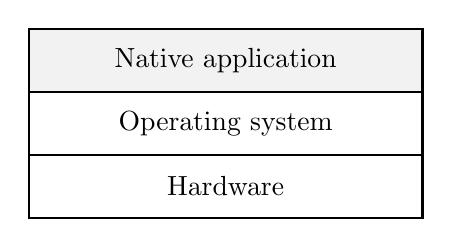
\begin{tikzpicture}[yscale=0.8]
    \fill[thick, black!5] (0,2) rectangle (5,3);
    \draw[thick] (0,0) rectangle (5,1);
    \draw[thick] (0,1) rectangle (5,2);
    \draw[thick] (0,2) rectangle (5,3);
    \node at (2.5,0.5) {Hardware};
    \node at (2.5,1.5) {Operating system};
    \node at (2.5,2.5) {Native application};
  \end{tikzpicture}
\caption{Native application}
\end{subfigure}%
\begin{subfigure}{0.5\textwidth}
  \centering
  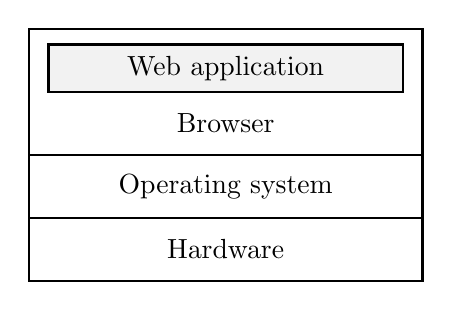
\begin{tikzpicture}[yscale=0.8]
    \fill[thick, black!5] (0.25,3) rectangle (4.75,3.75);
    \draw[thick] (0,0) rectangle (5,1);
    \draw[thick] (0,1) rectangle (5,2);
    \draw[thick] (0,2) rectangle (5,4);
    \draw[thick] (0.25,3) rectangle (4.75,3.75);
    \node at (2.5,0.5) {Hardware};
    \node at (2.5,1.5) {Operating system};
    \node at (2.5,2.5) {Browser};
    \node at (2.5,3.375) {Web application};
  \end{tikzpicture}
\caption{Web application}
\end{subfigure}
\caption{Native and web applications}
\label{fig:web-platform}
\end{figure}
\vspace*{-2em}

\subsection{Why WebAssembly?}

JavaScript has been the de facto language for web development since its introduction in 1995. Originally designed as a simple scripting language to bring interactivity to web pages, and famously built in just 10 days, JavaScript has been continuously extended to become the most widely used programming language in the world \cite{wirfs-brockJavaScriptfirst202020a}.

As web applications have increased in complexity, the consequences of JavaScript's complicated history have become more apparent. Being a high-level interpreted language, JavaScript is not well-suited for computationally intensive tasks. Similarly, its poor design as a language by modern standards, for example its lack of static typing, makes large codebases difficult to maintain \cite{ocarizajr.JavaScriptErrorsWild2011, biermanUnderstandingTypeScript2014}.

For these reasons, supporting other programming languages on the Web has been a much discussed topic. Early proprietary attempts, such as Java applets, ActiveX, and Flash, have all since been deprecated due to security concerns about running native code in the browser\footnote{Early attempts to support other programming languages on the Web allowed native code to be directly embedded into the web page, which proved very difficult to sufficiently ``sandbox''.}. More recently, Emscripten has been used to compile C and C++ code to a subset of JavaScript called asm.js, which is designed to be easily optimised by the JIT compilers of JavaScript engines \cite{zakaiEmscriptenLLVMtoJavaScriptcompiler2011}. While this approach mitigates many of the security concerns of the previous technologies, it remains inherently limited by the performance of JavaScript.

WebAssembly was introduced in 2017 as a solution to the problem of running safe, fast, portable, low-level code on the Web \cite{haasBringingwebspeed2017}. It is a binary instruction format for a stack-based virtual machine that is designed to be a compilation target for high-level languages, and able to run in the browser at near-native speed.

This section gives an overview of WebAssembly.

\subsection{Memory Model}

\label{sec:wasm-memory-model}

The WebAssembly specification \cite{rossbergWebAssemblyCoreSpecification2022} is very restrictive about how memory is accessed. The two areas of memory that are particularly relevant are the \emph{stack} and the \emph{linear memory}.

\paragraph{Stack}

A WebAssembly program executes as a \emph{stack machine}: operands of instructions are implicitly taken from the top of the stack, and results pushed back onto the stack. The stack also contains labels for control flow instructions, and \emph{activation frames} for function calls, which include local variables. Unlike the stack in a traditional programming language like C, the WebAssembly stack is not addressable; instead, local variables can only be referenced by their index from the stack pointer, meaning that stack-allocated variables cannot be passed to functions by reference. For example, in the C program below, the compiler must unintuitively allocate the local variable \texttt{x} in the linear memory, rather than on the stack, in order to pass it to the function \texttt{foo}.

\vspace*{-1em}

\begin{center}
\begin{minted}{c}
extern int foo(int*);
int main() {
  int x = 42;
  return foo(&x);
}
\end{minted}
\end{center}

\vspace*{-2em}

\paragraph{Linear Memory}

The main storage of a WebAssembly program is the \emph{linear memory}, or simply the \emph{memory}. It is a contiguous array of bytes, addressed by 32-bit pointers. These pointers are simply indices into the array, starting from zero (yes, zero is a valid address in WebAssembly). The memory is disjoint from the rest of the WebAssembly program. WebAssembly provides a \texttt{memory.grow} instruction to request that the host environment (e.g. the browser) increases the size of the contiguous memory area (an operation like \texttt{realloc}), however, there is no way to free memory.

\subsection{Interface with JavaScript}

\label{sec:wasm-js-interface}

A key design goal of WebAssembly is to be \emph{language-independent}, thus the WebAssembly specification makes no mention of JavaScript. Instead, it is up to the \emph{host environment} (e.g. the browser) to define and implement the necessary APIs for WebAssembly to interact with the outside world.

\paragraph{Import and Export} WebAssembly modules can import and export functions to and from the host environment, allowing JavaScript code to call WebAssembly functions, and vice versa. However, only integers and floats can be passed between the two environments in this way.

\paragraph{Shared Memory} To enable more complex data structures to be shared, the host environment exposes the WebAssembly module's linear memory to JavaScript as an array of bytes. This allows JavaScript code to serialise complex data structures into the linear memory, passing a pointer to the WebAssembly module, which can then access the data. WebAssembly functions can return complex data structures in the same way, illustrated in more detail in Appendix \ref{appendix:shared-memory}.

\section{Tools}

\label{sec:tools}

\paragraph{Rust}

Rust was chosen as the implementation language for the Prolog interpreter due to its strong support for WebAssembly and its focus on safety and performance. The officially-supported tool \texttt{wasm-bindgen} was used to facilitate interaction between Rust and JavaScript, alongside its companion tool \texttt{wasm-pack} for building and packaging the compiled WebAssembly module \cite{crichtonwasmbindgenhttpsgithubcom2014}.

\paragraph{Dependencies and Licensing}

Table \ref{tab:core-dependencies} lists the dependencies used in the implementation of the Prolog interpreter along with their licences, justifying the use of each one. Table \ref{tab:web-dependencies} lists the dependencies used in the implementation of the browser-based development environment.

\begin{table}[H]
\centering
\begin{tabular}{lll}
\hline
\textbf{Name} & \textbf{Licence} & \textbf{Justification} \\
\hline
\texttt{wasm-bindgen}$^*$ & MIT/Apache-2.0 & Calls between Rust and JavaScript \\
\texttt{wasm-pack}$^*$ & MIT/Apache-2.0 & Build and package WebAssembly module \\
\texttt{js-sys}$^*$ & MIT/Apache-2.0 & Bindings to JavaScript APIs \\
Serde & MIT/Apache-2.0 & Serialise and deserialise data \\
\texttt{serde-wasm-bindgen} & MIT & Rust-JavaScript data type conversion \\
LALRPOP & MIT/Apache-2.0 & Generate the parser \\
\hline
\end{tabular}
\caption{Dependencies of the interpreter. Dependencies marked with a * are officially supported by the Rust WebAssembly Working Group.}
\label{tab:core-dependencies}
\end{table}

\begin{table}[H]
\centering
\begin{tabular}{lll}
\hline
\textbf{Name} & \textbf{Licence} & \textbf{Justification} \\
\hline
React & MIT & JavaScript framework for building UI \\
Next.js & MIT & Compile React components to static HTML \\
\texttt{react-simple-code-editor} & MIT & Code editor component \\
Prism & MIT & Syntax highlighting \\
Iconoir & MIT & Icons \\
\hline
\end{tabular}
\caption{Dependencies of the browser-based development environment}
\label{tab:web-dependencies}
\end{table}

\paragraph{Version Control}

Git was used for version control, with the repository hosted on GitHub. Each phase of development was carried out on a separate branch, with pull requests used to merge completed features into the \texttt{main} branch.

\paragraph{Continuous Integration} GitHub Actions, a GitHub service to automatically run code on repository events, was used for continuous integration, compiling and running the test suite on each push to the repository. GitHub's ``branch protection'' feature was employed to ensure that commits to the \texttt{main} branch could only be made through pull requests, and that all checks must pass before merging.

\paragraph{Deployment} The browser-based development environment was automatically built and deployed to Cloudflare Pages, a static website hosting service, on each push to the \texttt{main} branch, again using GitHub Actions.

\section{Development Methodology}

\label{sec:dev-methodology}

The project was developed using a \emph{spiral} methodology \cite{boehmspiralmodelsoftware1986}, with development proceeding in a number of phases, each of which comprising requirements analysis, design, implementation, and testing. Evaluation in each phase involved quantitative comparison to existing Prolog implementations as described in Chapter 4, as well as qualitative comparison regarding feature completeness, which was then used to inform focus areas for the next phase.

The development phases were guided by the project proposal (Appendix \ref{appendix:proposal}), beginning with the implementation of a pure Prolog AST interpreter and building upon this.

The project was tested using a combination of unit tests, integration tests, and manual testing. Unit tests were written for each phase to ensure its correctness before proceeding to the next phase. The benchmarking suite, described in Chapter 4, also served as a form of integration testing, as it was run in the browser and required the correct functioning of the system as a whole, with each benchmark program additionally acting as a test case. Manual testing was used to evaluate the browser-based development environment.

\section{Requirements Analysis}

\label{sec:requirements}

The core requirements are stated in the project proposal (Appendix \ref{appendix:proposal}) and are as follows:

\vspace*{-1em}

\begin{quote}
``The project will be deemed a success if I have written a Prolog interpreter in Rust, compiled it to WebAssembly, and executed it in the browser, as well as having compared its performance with existing solutions, including SWI-Prolog compiled to WASM and Tau Prolog.''
\end{quote}

\vspace*{-1em}

In the proposal, a number of extensions were also suggested. Following the background research outlined in this chapter, several of these were selected to be implemented as extensions. This research also highlighted the importance of a garbage collector in a practical Prolog implementation, so this was added as a further extension.

\begin{itemize}
\setlength{\itemsep}{0em}
\item \textbf{Cut and Extra-Logical Predicates}: Implementing the cut operator and some extra-logical predicates, which are key components of a full Prolog implementation.
\item \textbf{Development Environment}: A browser-based development environment to demonstrate and evaluate the interpreter.
\item \textbf{Garbage Collection}: A garbage collector to improve memory efficiency.
\item \textbf{JavaScript FFI}: An FFI to improve integration with the browser.
\end{itemize}

\section{Starting Point}

\label{sec:starting-point}

As detailed in the project proposal (Appendix \ref{appendix:proposal}), I began the project from scratch, although with prior knowledge of Rust. I had little experience with Prolog, having only used it briefly in the Part IB Prolog course. No code was written before the beginning of Michaelmas Term 2024.

\chapter{Implementation}

This chapter gives an overview of the implementation of the project.

% TODO: overview

\section{Repository Overview}

\begin{table}[H]
\centering
\begin{tabular}{lp{11cm}l}
\hline
\textbf{Directory} & \textbf{Description} & \textbf{LOC} \\
\hline
\texttt{core/} & Implementation of the core interpreter in Rust, including the parser, garbage collector, and the JavaScript FFI. & TBD \\
\texttt{core/src/wasm} & WebAssembly interface for the core interpreter and JavaScript FFI. & \\
\texttt{core/src/tests} & Unit tests for the core interpreter. & \\
\texttt{lib/} & Higher-level JavaScript library for the interpreter. & \\
\texttt{web/} & Web-based development environment to demonstrate and benchmark the interpreter. & \\
\texttt{web/src/prolog} & TypeScript Prolog interface and wrappers for various Prolog interpreters. & \\
\texttt{bench/} & Web-based benchmarking tools. & \\
\texttt{docs/} & Documentation for the project. & \\
\hline
\end{tabular}
\caption{An overview of key directories in the repository}
\label{tab:repository-overview}
\end{table}

\section{Core Interpreter}

This section describes the implementation of the core Prolog interpreter, implemented in Rust.

\subsection{Memory Layout}

\label{sec:memory-layout}

The interpreter uses the merged heap/stack architecture proposed by Li \cite{liEfficientMemoryManagement2000} and described in Section \ref{sec:preparation-implementation}. Alongside the advantages identified by Li, notably improved cache performance, this architecture is uniquely suited to the linear memory model of WebAssembly.

In a traditional heap/stack architecture, the heap and stack are separate regions of memory, often with few constraints imposed on the layout of the heap. Indeed, SWI-Prolog simply uses \texttt{malloc} to allocate memory for terms on the heap\footnote{\url{https://www.swi-prolog.org/pldoc/man?section=memlimit}}, imposing no constraints on where the C runtime decides to put the memory. Running natively, this is not a problem, as virtual memory is plentiful. However, WebAssembly's linear memory is contiguous and limited in size, so the heap must be carefully managed by the WebAssembly code itself to avoid fragmentation. In addition, the trail stack contains pointers to bound variables, which may appear either on the stack or on the heap, but WebAssembly does not allow pointers to exist to stack-allocated objects. Therefore, the stack must also be placed in the linear memory, which further complicates memory management.

In a merged heap/stack architecture, all terms are allocated in one contiguous region of memory. This avoids the problem of fragmentation, as the heap grows with allocations and shrinks with instant reclaiming and garbage collection (Section \ref{sec:gc-impl}). If the heap grows too large for the linear memory, it suffices, in theory, to execute the \texttt{memory.grow} WebAssembly instruction, with no additional work from the WebAssembly module required. In my implementation, the exact placement of the heap in the linear memory is decided by Rust's allocator, but once the heap grows sufficiently large, this has the same effect (Section \ref{sec:heap-placement}).

Of course, other areas of memory are needed:

\paragraph{Trail Stack} The trail stack is a stack of pointers to variables that have been bound, used for backtracking.

\paragraph{Choice Point Stack} The choice point stack stores information about where to backtrack to for each choice we make. Alongside the next clause to consider, each choice point also contains the sizes of the heap, trail stack and goal stack to facilitate backtracking and instant reclaiming.

\paragraph{Goal Stack} The goal stack contains the remaining goals to prove. When backtracking, goals that have previously been popped might be needed again, so while I refer to it as a stack, the goal stack is actually a graph, with goals represented as pairs $(\texttt{pred}, \texttt{goal})$ and the goal stack additionally storing a pointer to the current goal (the ``top of the stack'').

\begin{figure}[H]
\centering
\begin{subfigure}{.5\textwidth}
\centering
\begin{minted}{prolog}
a(1).
a(2).
b(2).
?- a(X), b(X).

\end{minted}
\caption{A Prolog program}
\end{subfigure}%
\begin{subfigure}{.5\textwidth}
\centering
\begin{tikzpicture}
  \node (A) at (0,3) {\mintinline{prolog}{a(X), b(X)}};
  \node (B1) at (-2,1.5) {\mintinline{prolog}{b(1)}};
  \node (B2) at (2,1.5) {\mintinline{prolog}{b(2)}};
  \node (C2) at (2,0) {\{\}};

  \draw (A) -- (B1) node [midway, xshift=-30, yshift=4] {\footnotesize \texttt{X = 1}};
  \draw (A) -- (B2) node [midway, xshift=30, yshift=4] {\footnotesize \texttt{X = 2}};
  \draw (B2) -- (C2);

  \node (D) at (-2,1) {\footnotesize (failure)};
\end{tikzpicture}
\caption{Corresponding SLD-tree}
\end{subfigure}
\par\bigskip
\par\bigskip
\begin{subfigure}{.5\textwidth}
\centering
\begin{tikzpicture}[box/.style={draw, rectangle}]
  \node[box] (B) at (0, 0) {\mintinline{prolog}{b(X)}};
  \node[box] (A) at (3, 0) {\mintinline{prolog}{a(X)}};

  \node (null) at (-2, 0) {\texttt{null}};
  \node (current) at (0, 2) {current goal};
  \node (cp1) at (3, 2.5) {choice point};
  \node (cp2) at (3, 2) {goal pointer};

  \draw[->] (A) -- (B);
  \draw[->] (B) -- (null);
  \draw[->] (current) -- (A);
  \draw[->] (cp2) -- (A);
\end{tikzpicture}
\vspace{5mm}
\caption{The goal graph before the first resolution}
\end{subfigure}%
\begin{subfigure}{.5\textwidth}
\centering
\begin{tikzpicture}[box/.style={draw, rectangle}]
  \node[box] (B) at (0, 0) {\mintinline{prolog}{b(X)}};
  \node[box, fill=lightgray] (A) at (3, 0) {\mintinline{prolog}{a(X)}};

  \node (null) at (-2, 0) {\texttt{null}};
  \node (current) at (0, 2) {current goal};
  \node (cp1) at (3, 2.5) {choice point};
  \node (cp2) at (3, 2) {goal pointer};

  \draw[->] (A) -- (B);
  \draw[->] (B) -- (null);
  \draw[->] (current) -- (B);
  \draw[->] (cp2) -- (A);
\end{tikzpicture}
\vspace{5mm}
\caption{The goal graph after the first resolution}
\end{subfigure}
\vspace*{-5mm}
\caption{The goal graph}
\label{fig:goals}
\end{figure}

Figure \ref{fig:goals} illustrates this idea. Before resolving \mintinline{prolog}{a(X)} with \mintinline{prolog}{a(1)} (c), a choice point is created, containing a pointer to the current goal. After the resolution step, \mintinline{prolog}{a(X)} is ``popped from the goal stack'', which is implemented by setting the current goal pointer to its predecessor (d). Importantly, however, it remains in the graph, as upon backtracking to the choice point when \mintinline{prolog}{b(1)} fails, the current goal pointer is restored to that stored in the choice point. In order to prevent the goal stack growing indefinitely, each choice point also contains the number of goals in the stack when it was created, and the goal stack is truncated to this size upon backtracking. The goal stack is also garbage collected (Section \ref{sec:gc-impl}).

\paragraph{Code Area} There is no separate code area, as the clauses of the program are stored on the heap using the same representation as regular terms, an idea suggested by Tarau \cite{tarauHitchhikersGuideReinventing2018}. Initially, my implementation did use a distinct code area with a different representation, but profiling revealed that, in the former implementation, up to 40\% of the execution time was spent copying terms onto the heap. Benchmarking confirmed that Tarau's approach reduced execution time by around 25\% across various benchmarks (Section \ref{sec:benchmarking}).

In this implementation, copying a clause onto the heap when a goal unifies with its head consists of a single \texttt{memcpy} followed by a linear scan of the copied clause terms to add the appropriate offset to any pointers. To efficiently identify the byte boundaries between terms in the body of the clause, each clause additionally includes a ``header'' containing $n$ variables, bound to each of the $n$ terms in its body.

\subsection{Pointers}

A common theme in the implementation of this project, taken from WebAssembly, is that of using indexing over pointers. The contiguous nature of the heap allows terms to be referred to by their index, and the same is true for the goal stack and choice point stack.

Rust strongly discourages the use of raw pointers, instead preferring its memory-safe abstraction, references. Every object in Rust must have exactly one \emph{owner}, with multiple immutable references or a single mutable reference allowed, enforced at compile time by the \emph{borrow checker}. The Prolog heap does not fit nicely into this model: there may be multiple variables bound to the same term, both of which requiring mutable access to it (e.g. to update the term when unifying). One way to work around this is to use reference counting and \texttt{RefCell}, which facilitates runtime borrow checking, but this is very expensive in terms of performance. Instead, terms are referred to by their index in the heap. As we use a merged heap/stack architecture, this is straightforward to implement. Hereafter, any references to ``pointers to heap terms'' actually mean indices.

The performance consequences of these approaches are discussed in more detail in Section \ref{sec:get-unchecked}.

\subsection{Term Representation}

Terms are stored on the heap as fixed-size blocks of 24 bytes. In Rust, these are represented as an enum (Figure \ref{fig:rust-term-representation}), Rust's sum type.

Atoms are typed, being either strings, integers, or floats, with implicit casting from integers to floats permitted. The representation of variables includes a pointer to their bound object, as in the WAM, but additionally a boolean flag to indicate whether they are \emph{shunted} (Section \ref{sec:variable-shunting}), which is used in garbage collection. Compound terms, represented by their functor and arity $n$, are followed in the heap by $n$ variables pointing to each of their arguments. There is also a heap representation of cut, which is necessary because goals are stored on the heap. Finally, \emph{lambda terms}, used to call JavaScript code from within the Prolog execution (Section \ref{sec:js-ffi}), are represented in the same way as compound terms, except instead of storing a functor, they store the raw JavaScript code.

All other kinds of term supported in the Prolog syntax are syntactic sugar for terms represented as above, converted during parsing. For example, the arithmetic expression $2 + 3$ becomes the compound term \texttt{+(2, 3)}, and the list \texttt{[a, b]} becomes the compound term \texttt{.(a, .(b, []))}.

\begin{figure}[H]
\centering
\begin{subfigure}{0.5\textwidth}
\centering
\begin{minted}{rust}
pub enum HeapTerm {
    Atom(Atom),
    Var(HeapTermPtr, bool),
    Compound(StringId, usize),
    Cut(ChoicePointIdx),
    Lambda(StringId, usize),
}
\end{minted}
\end{subfigure}%
\begin{subfigure}{0.5\textwidth}
\centering
\begin{minted}{rust}
pub enum Atom {
    String(StringId),
    Integer(i64),
    Float(f64),
}


\end{minted}
\end{subfigure}
\caption{Term representation in Rust}
\label{fig:rust-term-representation}
\end{figure}

\subsection{Parsing}

The Prolog program is parsed into its abstract syntax tree (AST) using a parser generated by LALRPOP \cite{thelalrpopprojectdevelopersLALRPOPhttpsgithubcom2015} with a custom grammar, written from scratch.

\begin{figure}[H]
\centering
\begin{minted}{rust}
Clause: Clause = {
    <h:Term> "." => Clause(h, vec![]),
    <h:Term> ":-" <b:Comma<Term>> "." => Clause(h, b),
}
Comma<T>: Vec<T> = {
    <t:T> => vec![t],
    <mut ts:Comma<T>> "," <t:T> => { ts.push(t); ts },
}
\end{minted}
\caption{Extract from the LALRPOP grammar}
\label{fig:grammar}
\end{figure}

Figure \ref{fig:grammar} shows an extract from the grammar. LALRPOP supports polymorphic non-terminals, which are used in the extract to define a generic non-empty comma-separated list of terms, \texttt{Comma<T>}. The \texttt{vec!} macro is used to create a vector using array-like syntax.

\subsection{Built-in Predicates}

\label{sec:builtins}

In order to do useful computation, the interpreter must support a set of built-in predicates, such as arithmetic evaluation. The full list of built-in predicates is given in Appendix \ref{appendix:predicates}.

Each predicate implements a \emph{trait} called \texttt{Builtin}, which is similar to an interface in C++ or Java. The definition of this trait is shown in Figure \ref{fig:builtin-trait}. This trait has an associated constant, \texttt{ARITY}, which is the number of arguments the predicate takes. A pointer to the first argument is passed to the \texttt{eval} function. This function evaluates the predicate, potentially modifying the state of the interpreter through the mutable reference to the \texttt{Solver} object, returning a boolean if the predicate succeeded or failed with no errors, or an error otherwise, for example if an argument was insufficiently instantiated.

\begin{figure}[H]
\centering
\begin{minted}{rust}
pub trait Builtin<const ARITY: usize> {
    fn eval(solver: &mut Solver, args: HeapTermPtr)
        -> Result<bool, BuiltinError>;
}
\end{minted}
\caption{The \texttt{Builtin} trait}
\label{fig:builtin-trait}
\end{figure}

Many built-in predicates are implemented almost identically, for example the extra-logical type testing predicates \texttt{var/1}, \texttt{atom/1}, and \texttt{integer/1} (among others), which only differ in the type they compare against. To avoid code duplication, these predicates are implemented using meta-programming, with a \emph{macro} generating the code for each type. Figure \ref{fig:builtin-macro} shows the macro for type testing predicates. It uses Rust's pattern matching syntax to match the heap representation of the term against a pattern \texttt{\$matcher} representing the type to check for.

\begin{figure}[H]
\centering
\begin{minted}{rust}
macro_rules! impl_type_check {
    ($name:ident, $matcher:pat) => {
        pub struct $name;
        impl Builtin<1> for $name {
            fn eval(solver: &mut Solver, args: HeapTermPtr)
                -> Result<bool, BuiltinError>
            {
                Ok(matches!(solver.heap.get(args), $matcher))
            }
        }
    };
}

impl_type_check!(IsIntegerBuiltin, HeapTerm::Atom(Atom::Integer(_)));
impl_type_check!(IsAtomBuiltin, HeapTerm::Atom(_));
impl_type_check!(IsVarBuiltin, HeapTerm::Var(_, _));
\end{minted}
\caption{Macro for type testing predicates}
\label{fig:builtin-macro}
\end{figure}

\subsection{Cut}

The cut operator, \texttt{!/0}, is an extra-logical predicate that commits to the clause in which it appears. In other words, backtracking past a cut causes the clause it appears in to fail.

When a clause is copied onto the heap, a linear scan updates its variables by the appropriate offset (Section \ref{sec:memory-layout}). This linear scan also updates the heap representations of any instances of the cut operator to include the index of the current choice point, that is, the choice point before this clause was selected. When the cut operator becomes the current goal, the choice point stack is truncated to the choice point it refers to.

\section{Optimisations}

\subsection{Choice Point Elimination (incl. Last Call Optimisation)}

Last call optimisation (LCO) is traditionally implemented by reusing the stack frame for the last call of a determinate predicate (Section \ref{sec:preparation-implementation}). This is only applicable on the final clause of a predicate, as otherwise the predicate would not be determinate.

However, in my implementation, we do not have a call stack, instead storing all terms on the heap and using a goal stack and choice point stack for control (Section \ref{sec:memory-layout}). Therefore, it is not the call stack that grows indefinitely, but the choice point stack. I implement a variant of last call optimisation, which I call \emph{choice point elimination}. This works by not creating a choice point for the final clause of a predicate, as its failure necessarily implies the failure of the entire predicate. Static analysis prior to execution is required to group clauses into predicates to enable this optimisation.

Instead of reusing the stack frame on the call stack, TODO

\subsection{String Interning}

Strings are expensive to copy because they must be dynamically allocated in the linear memory. Comparing two strings for equality is also orders of magnitude more expensive than a simple arithmetic comparison, requiring both memory reads and $O(n)$ comparisons (where $n$ is the length of the string), as opposed to a single WebAssembly instruction for arithmetic comparison.

For this reason, the implementation avoids using \texttt{String} objects wherever possible by using \emph{string interning}. All strings are allocated in a specific area of memory, and all references to each string are replaced with its index in that area. A hash table, mapping strings to their indices, is used to ensure that no duplicate strings appear.

A further optimisation initialises the string area with fixed mappings for commonly-used strings, such as the names of built-in predicates and arithmetic operators. For example, the string \texttt{"+"} is always at index 9, stored as a constant \texttt{str::ADD} in the Rust code, so a real string comparison is not necessary, even with runtime-generated strings (due to the uniqueness of string mapping). Figure \ref{fig:fixed-string-indices} shows how this is used in the arithmetic evaluation code (simplified).

\begin{figure}[H]
\centering
\begin{subfigure}{.5\textwidth}
\centering
\begin{minted}{rust}
match functor {
    str::ADD /*  9 */ => add(&a, &b),
    str::SUB /* 10 */ => sub(&a, &b),
    str::MUL /* 11 */ => mul(&a, &b),
    str::DIV /* 12 */ => div(&a, &b),
    ...
}
\end{minted}
\caption{Arithmetic comparison of functors}
\end{subfigure}%
\begin{subfigure}{.5\textwidth}
\centering
\begin{minted}{rust}
match functor {
    "+" => add(&a, &b),
    "-" => sub(&a, &b),
    "*" => mul(&a, &b),
    "/" => div(&a, &b),
    ...
}
\end{minted}
\caption{String comparison of functors}
\end{subfigure}
\caption{Using fixed string indices for arithmetic evaluation}
\label{fig:fixed-string-indices}
\end{figure}

\section{Garbage Collection}

\label{sec:gc-impl}

\section{JavaScript FFI}

\label{sec:js-ffi}

\section{Web-Based Development Environment}

%TC:group table 0 1
%TC:group tabular 1 1

\chapter{Evaluation}

This chapter evaluates the performance of WebPL in terms of execution time (Section~\ref{sec:execution-time}), memory usage (Section~\ref{sec:memory-usage}), and binary size (Section~\ref{sec:binary-size}), and compares it to existing Prolog implementations for the Web. Then, factors contributing to the performance differences are explored, and possible improvements to SWI-Prolog are described (Section~\ref{sec:swi-prolog-optimisation}). Finally, the use of the Rust programming language is evaluated (Section~\ref{sec:rust-evaluation}).

\section{Benchmark Programs}

A subset of the SWI-Prolog benchmark suite \cite{wielemakerSWIPrologbenchmarksuite2010}, itself derived from a collection of widely-used Prolog benchmarks \cite{haygoodPrologBenchmarkSuite1989}, was selected to evaluate the performance of WebPL. This consists of 16 benchmarks, excluding the 19 which use features not supported in WebPL.

The benchmarks selected for this evaluation cover a range of tasks, including parsing natural language, symbolic differentiation, list manipulation, arithmetic, and solving puzzles such as the 8-Queens problem. The full benchmark suite is detailed in Appendix~\ref{appendix:benchmarks}.

\section{Execution Time}

\label{sec:execution-time}

The implementation-agnostic TypeScript interface, developed as part of the browser-based development environment (Section~\ref{sec:prolog-interface}), was further used to build an in-browser benchmarking tool.

Each benchmark was initially run up to 20 times or for 100ms, whichever was shorter, to populate the cache. Then, during the measurement phase, each benchmark was run at least 10 more times, for a maximum of 1000 runs or 5 seconds of benchmarking. The execution time of each run was measured using the browser's \texttt{performance.now()} function, which provides high-resolution timestamps. However, high-resolution timestamps are only available in \emph{secure contexts} for security reasons \cite{sanchez-rolaClockClockTimeBased2018}, so the benchmarking tool was hosted on a local server configured to use HTTPS.

Benchmarks were run in Chrome 134 on a MacBook Pro with an Apple M3 Pro chip and 18GB of RAM, running macOS 15.3 (Sequoia).

\subsection{Comparison of Prolog Implementations}

\label{sec:prolog-comparison}

Table~\ref{tab:chrome-time} shows the median execution time of each benchmark for each implementation tested.

\begin{table}[H]
\centering
\setstretch{1}
\begin{tabular}{lrrrrr}
\addlinespace\hline\addlinespace
Benchmark & WebPL & WebPL+GC & SWI & Trealla & Tau \\
\addlinespace\hline\addlinespace
chat\_parser  & \green{17.22}  &  18.51  &  74.44  &  26.90  &  1610.90  \\
crypt        &   0.64  &   \green{0.63}  &   3.00  &   3.62  &   120.77  \\
derive       &   0.29  &   \green{0.28}  &   1.20  &   0.45  &    13.25  \\
divide10     &   0.27  &   \green{0.24}  &   1.08  &   0.39  &    12.99  \\
fib          &   \green{4.84}  &   7.41  &   9.72  &   5.08  &  3040.73  \\
log10        &   \green{0.27}  &   \green{0.27}  &   1.08  &   0.41  &    13.40  \\
mu           &   \green{0.34}  &   0.36  &   1.32  &   0.62  &    15.03  \\
nreverse     &   \green{0.29}  &   0.38  &   0.65  &   0.40  &    17.28  \\
ops8         &   0.28  &   \green{0.27}  &   1.10  &   0.46  &    13.18  \\
poly\_10      &   \green{5.48}  &  16.98$^*$\hspace{-0.4em}  &  19.31  &   6.45  &  3481.89  \\
qsort        &   \green{0.32}  &   0.38  &   0.84  &   0.55  &    18.12  \\
queens\_8     &   \green{6.49}  &   7.30  &  17.87  &   8.38  &   267.43  \\
query        &  \green{0.77}  &   0.82  &   2.68  &   1.26  &    20.31  \\
tak          &  \green{15.33}  &  38.56$^*$\hspace{-0.4em}  &  28.20  &  27.96  & 26691.83  \\
times10      &   \green{0.27}  &   \green{0.27}  &   1.14  &   0.57  &    12.88  \\
zebra        &   3.16  &   \green{3.13}  &   7.82  &   9.76  &   901.52  \\
\addlinespace\hline\addlinespace
\end{tabular}
\caption{Execution time of benchmarks (milliseconds)}
\label{tab:chrome-time}
\end{table}

\vspace*{-1.5em}

Unexpectedly, but pleasingly, the results show that WebPL is faster than all other Prolog implementations tested in every benchmark without garbage collection, and all but two when garbage collection is enabled (marked with a $\ast$). Section~\ref{sec:swi-prolog-optimisation} explores why this is, and how some modifications to the SWI-Prolog build process can make its execution time more competitive.

\begin{figure}[H]
\centering
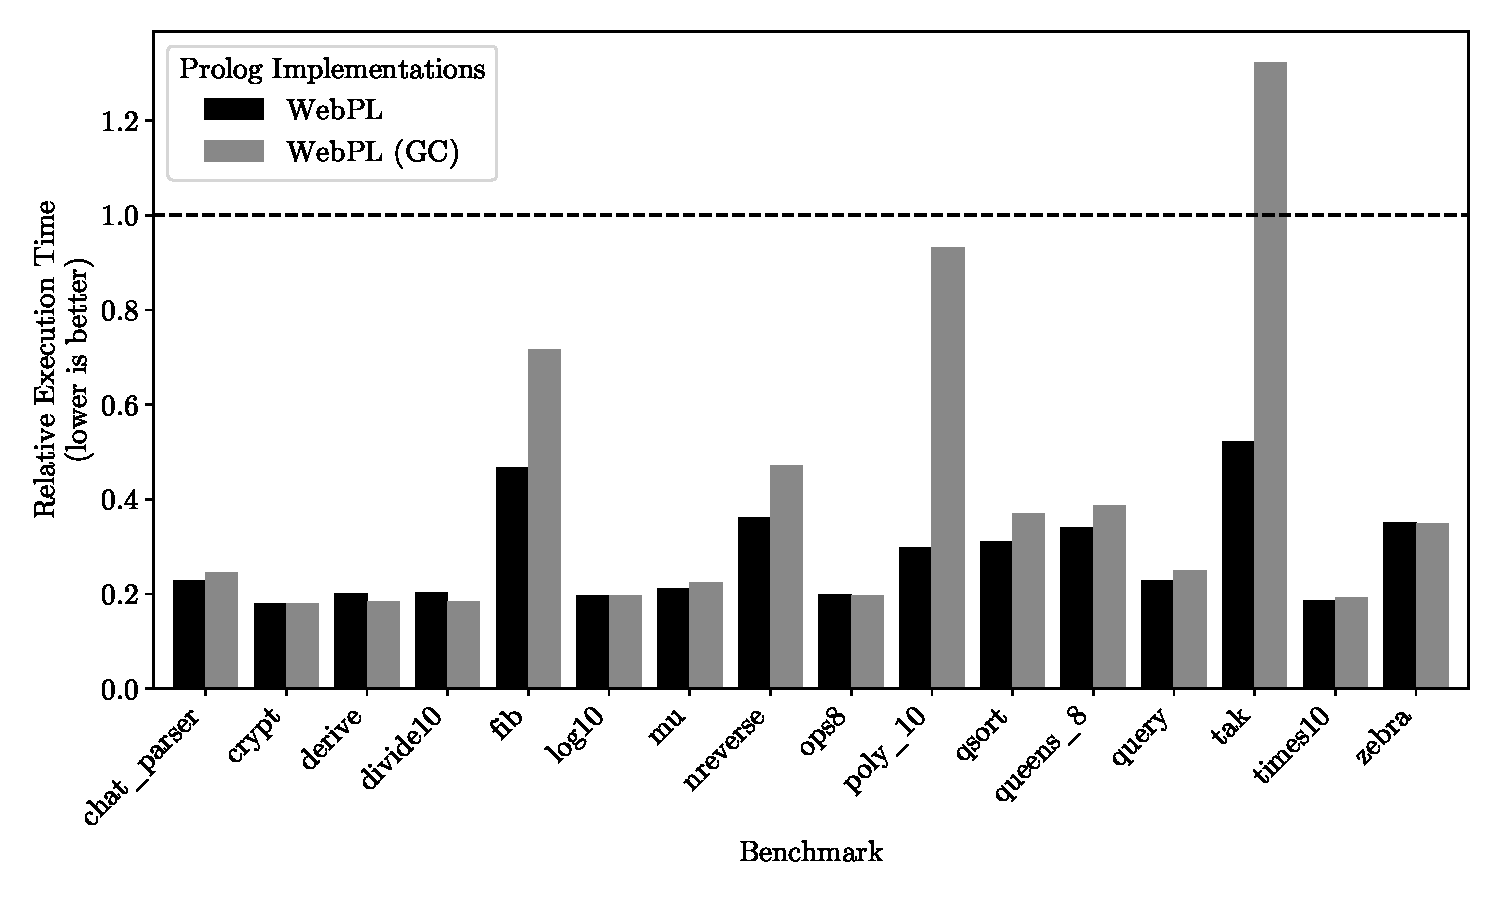
\includegraphics[width=0.8\textwidth]{relative_performance.pdf}
\caption{Execution time of benchmarks relative to SWI-Prolog}
\label{fig:relative-performance}
\end{figure}

Figure~\ref{fig:relative-performance} shows the execution time of WebPL, relative to SWI-Prolog, based on the same data as Table~\ref{tab:chrome-time}, with error bars representing quartiles.

This reveals that for three benchmarks, \texttt{fib}, \texttt{poly\_10}, and \texttt{tak}, garbage collection has a major impact on performance, increasing execution time by 53\%, 210\%, and 152\% respectively. These benchmarks are the most memory-intensive, so garbage collection runs more frequently, decreasing performance.

The WebPL garbage collection scheduler invokes the garbage collector whenever heap utilisation exceeds a certain threshold (by default, 90\%). If this does not reduce heap utilisation below the threshold, garbage collection is not invoked again until the threshold is met again after the heap has been resized, which occurs when it is completely full. Furthermore, after a garbage collection, there is a timeout before another can begin, to avoid invoking garbage collection too frequently.

This is a more aggressive strategy than that of SWI-Prolog, which does not consider the allocated size of the heap when deciding when to invoke the garbage collector, instead considering the used size of the heap at the last garbage collection\footnote{\url{https://www.swi-prolog.org/pldoc/man?section=gc}}. Therefore, SWI-Prolog is less conservative of memory (Section~\ref{sec:memory-usage}), and may resize the heap unnecessarily, but avoids the performance penalty of frequent garbage collections.

\section{Memory Usage}

\label{sec:memory-usage}

A notable criticism of existing Prolog implementations for the Web is their high memory usage (Section~\ref{sec:motivation}).

Two approaches were taken in evaluating memory usage. The browser's \texttt{performance.memory} API was used to measure the memory usage of a browser tab running the Prolog implementation (Section~\ref{sec:web-page-memory-usage}). However, this includes the size of the WebAssembly binary, located in the memory of the tab. Therefore, the implementation's own memory usage statistics were also used, but this is only available in WebPL and SWI-Prolog (Section~\ref{sec:prolog-heap-usage}).

\subsection{Web-Page Memory Usage}

\label{sec:web-page-memory-usage}

To evaluate the memory usage of each Prolog implementation for each benchmark, a Python script using the Selenium browser automation library \cite{softwarefreedomconservancySeleniumhttpsgithubcom2025} was developed. For each implementation and each benchmark, the script starts a new browser instance, loads the implementation and benchmark, runs the benchmark once, and measures the memory usage of the tab using \texttt{performance.memory}. As memory used by WebAssembly cannot be freed, the resulting measurement is the peak memory usage during the execution of the benchmark (Table~\ref{tab:chrome-memory}).

\begin{table}[H]
\centering
\setstretch{1}
\begin{tabular}{lrrrrr}
\addlinespace\hline\addlinespace
Benchmark & WebPL & WebPL+GC & SWI & Trealla & Tau \\
\addlinespace\hline\addlinespace
chat\_parser & 6.02 & \green{5.58} & 36.57 & 26.05 & 83.05 \\
crypt & \green{4.90} & \green{4.90} & 36.71 & 25.10 & 29.72 \\
derive & \green{4.90} & \green{4.90} & 36.95 & 25.09 & 5.71 \\
divide10 & \green{4.90} & \green{4.90} & 36.45 & 25.09 & 5.46 \\
fib & 36.77 & \green{5.33} & 36.20 & 31.78 & 679.96 \\
log10 & \green{4.90} & \green{4.90} & 36.70 & 25.09 & 5.46 \\
mu & \green{4.90} & \green{4.90} & 36.45 & 25.09 & 5.96 \\
nreverse & \green{4.89} & \green{4.89} & 36.45 & 25.21 & 9.46 \\
ops8 & \green{4.90} & \green{4.90} & 36.45 & 25.09 & 5.46 \\
poly\_10 & 36.78 & \green{5.22} & 36.71 & 35.84 & 227.97 \\
qsort & \green{4.89} & 4.90 & 36.20 & 25.22 & 7.03 \\
queens\_8 & \green{4.90} & \green{4.90} & 36.46 & 25.10 & 69.47 \\
query & \green{4.90} & \green{4.90} & 36.71 & 25.33 & 5.72 \\
tak & 133.39 & \green{36.89} & 41.01 & 87.20 & 3186.35 \\
times10 & \green{4.90} & \green{4.90} & 36.45 & 25.09 & 5.46 \\
zebra & \green{4.90} & \green{4.90} & 36.45 & 25.10 & 104.97 \\
\addlinespace\hline\addlinespace
\end{tabular}
\caption{Memory usage of benchmarks (megabytes)}
\label{tab:chrome-memory}
\end{table}

WebPL shows the lowest memory usage for all benchmarks with garbage collection enabled. However, the variance of memory usage across benchmarks is very small due to the often much larger binary size being included. To better evaluate the memory usage of the Prolog implementations themselves, another approach was taken.

\subsection{Prolog Heap Usage}

\label{sec:prolog-heap-usage}

WebPL, like SWI-Prolog, provides a built-in \texttt{statistics/2} predicate to access statistics about the execution. One such statistic is the allocated size of the Prolog heap. By adding this predicate to the end of the query to be benchmarked, the memory usage of the Prolog implementation itself can be measured. Figure~\ref{fig:heap-usage} shows the allocated heap size of WebPL with garbage collection enabled for each benchmark, relative to that of SWI-Prolog.

\begin{figure}[t]
\centering
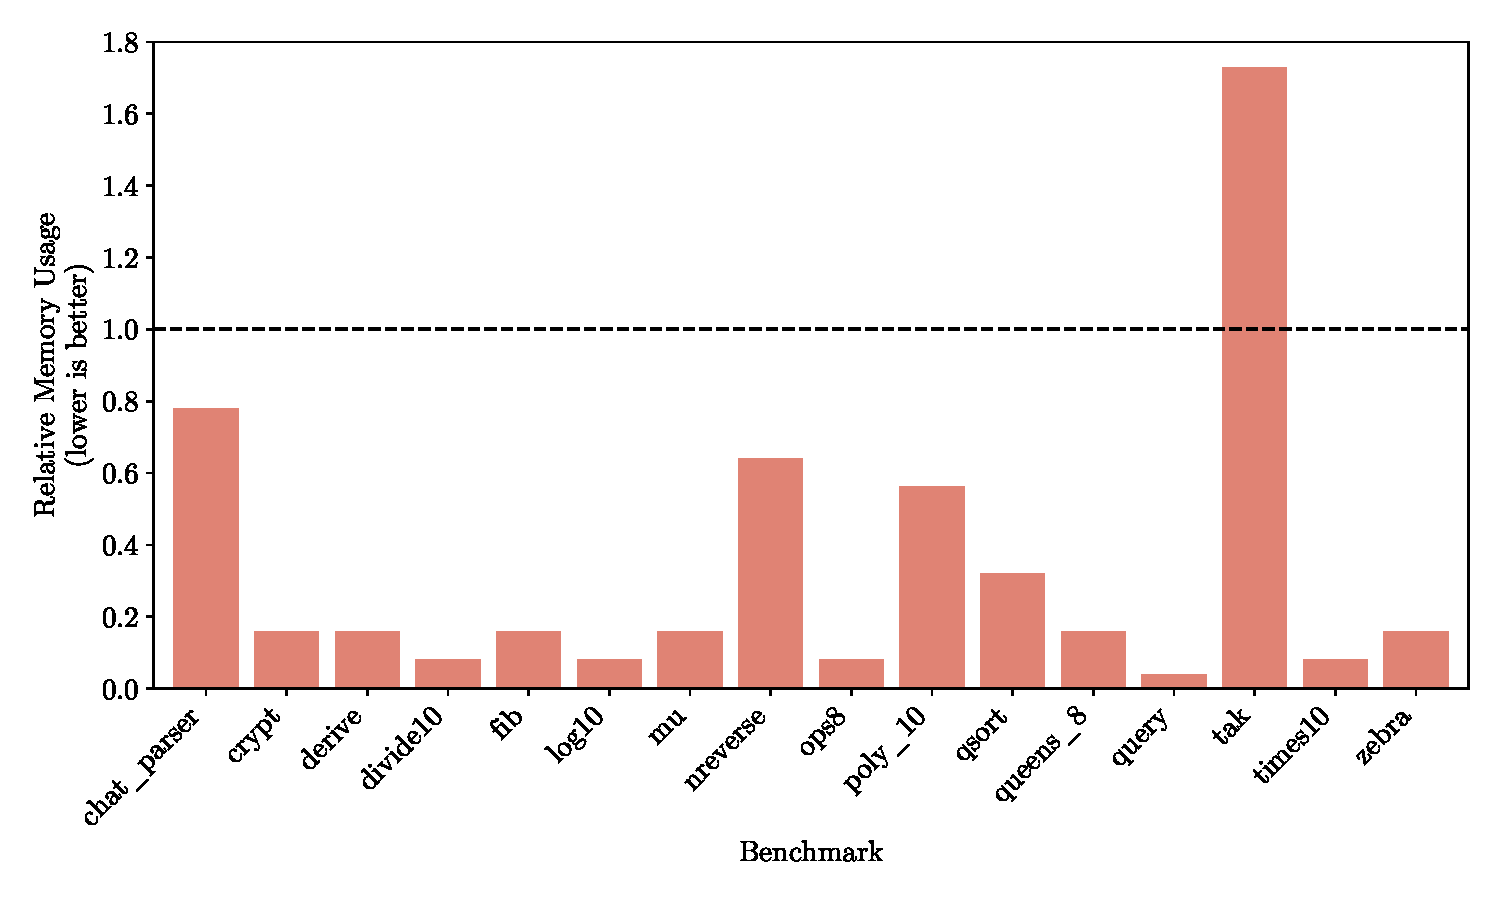
\includegraphics[width=0.8\textwidth]{relative_memory_builtin.pdf}
\caption{WebPL (GC) allocated heap size relative to SWI-Prolog}
\label{fig:heap-usage}
\end{figure}

For some benchmarks, WebPL uses much less memory than SWI-Prolog. This is because SWI-Prolog pre-allocates a fixed amount of heap memory to avoid the overhead of doing so during execution, while WebPL does not, instead doubling the size of the heap each time it gets full. As a result, WebPL never allocates more than twice the memory it needs.

For other benchmarks, WebPL uses slightly less memory than SWI-Prolog. Only in the case of \texttt{tak} does WebPL use more. These are the more memory-intensive benchmarks, possibly indicating that, in the limit, SWI-Prolog is more memory-efficient. The use of Rust for WebPL limits the memory usage optimisations that can be made (Section~\ref{sec:rust-evaluation}).

\section{Binary Size}

\label{sec:binary-size}

Another important consideration for any web application is how much data needs to be downloaded to the client. Unlike native applications, which are downloaded once and run locally, web applications are usually loaded from the server every time a client visits the page. Therefore, the size of the application can have a significant impact on the time it takes to load the page, especially on mobile devices with slower connections. This is a common weakness of WebAssembly applications, as WebAssembly binaries can be large, often due to the inclusion of libraries, such as \texttt{libc}, which, unlike in native applications, cannot be dynamically linked.

Table~\ref{tab:binary-size} shows the size of the WebAssembly binary (for WebPL, SWI-Prolog, and Trealla Prolog) or the JavaScript bundle (for Tau Prolog) for each Prolog implementation.

\begin{table}[H]
\centering
\begin{tabular}{ll}
\addlinespace\hline\addlinespace
Implementation & Binary/Bundle Size \\
\addlinespace\hline\addlinespace
WebPL & 0.84 MB \\
SWI-Prolog & 7.95 MB \\
Trealla Prolog & 4.48 MB \\
Tau Prolog & \green{0.57 MB} \\
\addlinespace\hline\addlinespace
\end{tabular}
\caption{Binary/bundle size of Prolog implementations (megabytes)}
\label{tab:binary-size}
\end{table}

While Tau Prolog, written in JavaScript, is the smallest, WebPL is the only WebAssembly implementation smaller than 1MB, and is only 48\% larger than Tau Prolog, significantly less than SWI-Prolog and Trealla Prolog. Section~\ref{sec:binary-size-opt} explores why SWI-Prolog is so large, and how its size can be reduced.

\section{SWI-Prolog Optimisation}

\label{sec:swi-prolog-optimisation}

Given the unexpectedly poor performance of industry-standard SWI-Prolog in both execution time and binary size, I explored why this may be, and made some optimisations.

\subsection{Profiling SWI-Prolog}

As identified in Section~\ref{sec:prolog-comparison}, WebPL's execution time is significantly faster than that of SWI-Prolog. To explore why, I profiled the execution of the \texttt{queens\_8} benchmark in SWI-Prolog using Chrome DevTools. Figure~\ref{fig:swi-prolog-profile} shows the resulting stack chart.

\begin{figure}[H]
\centering
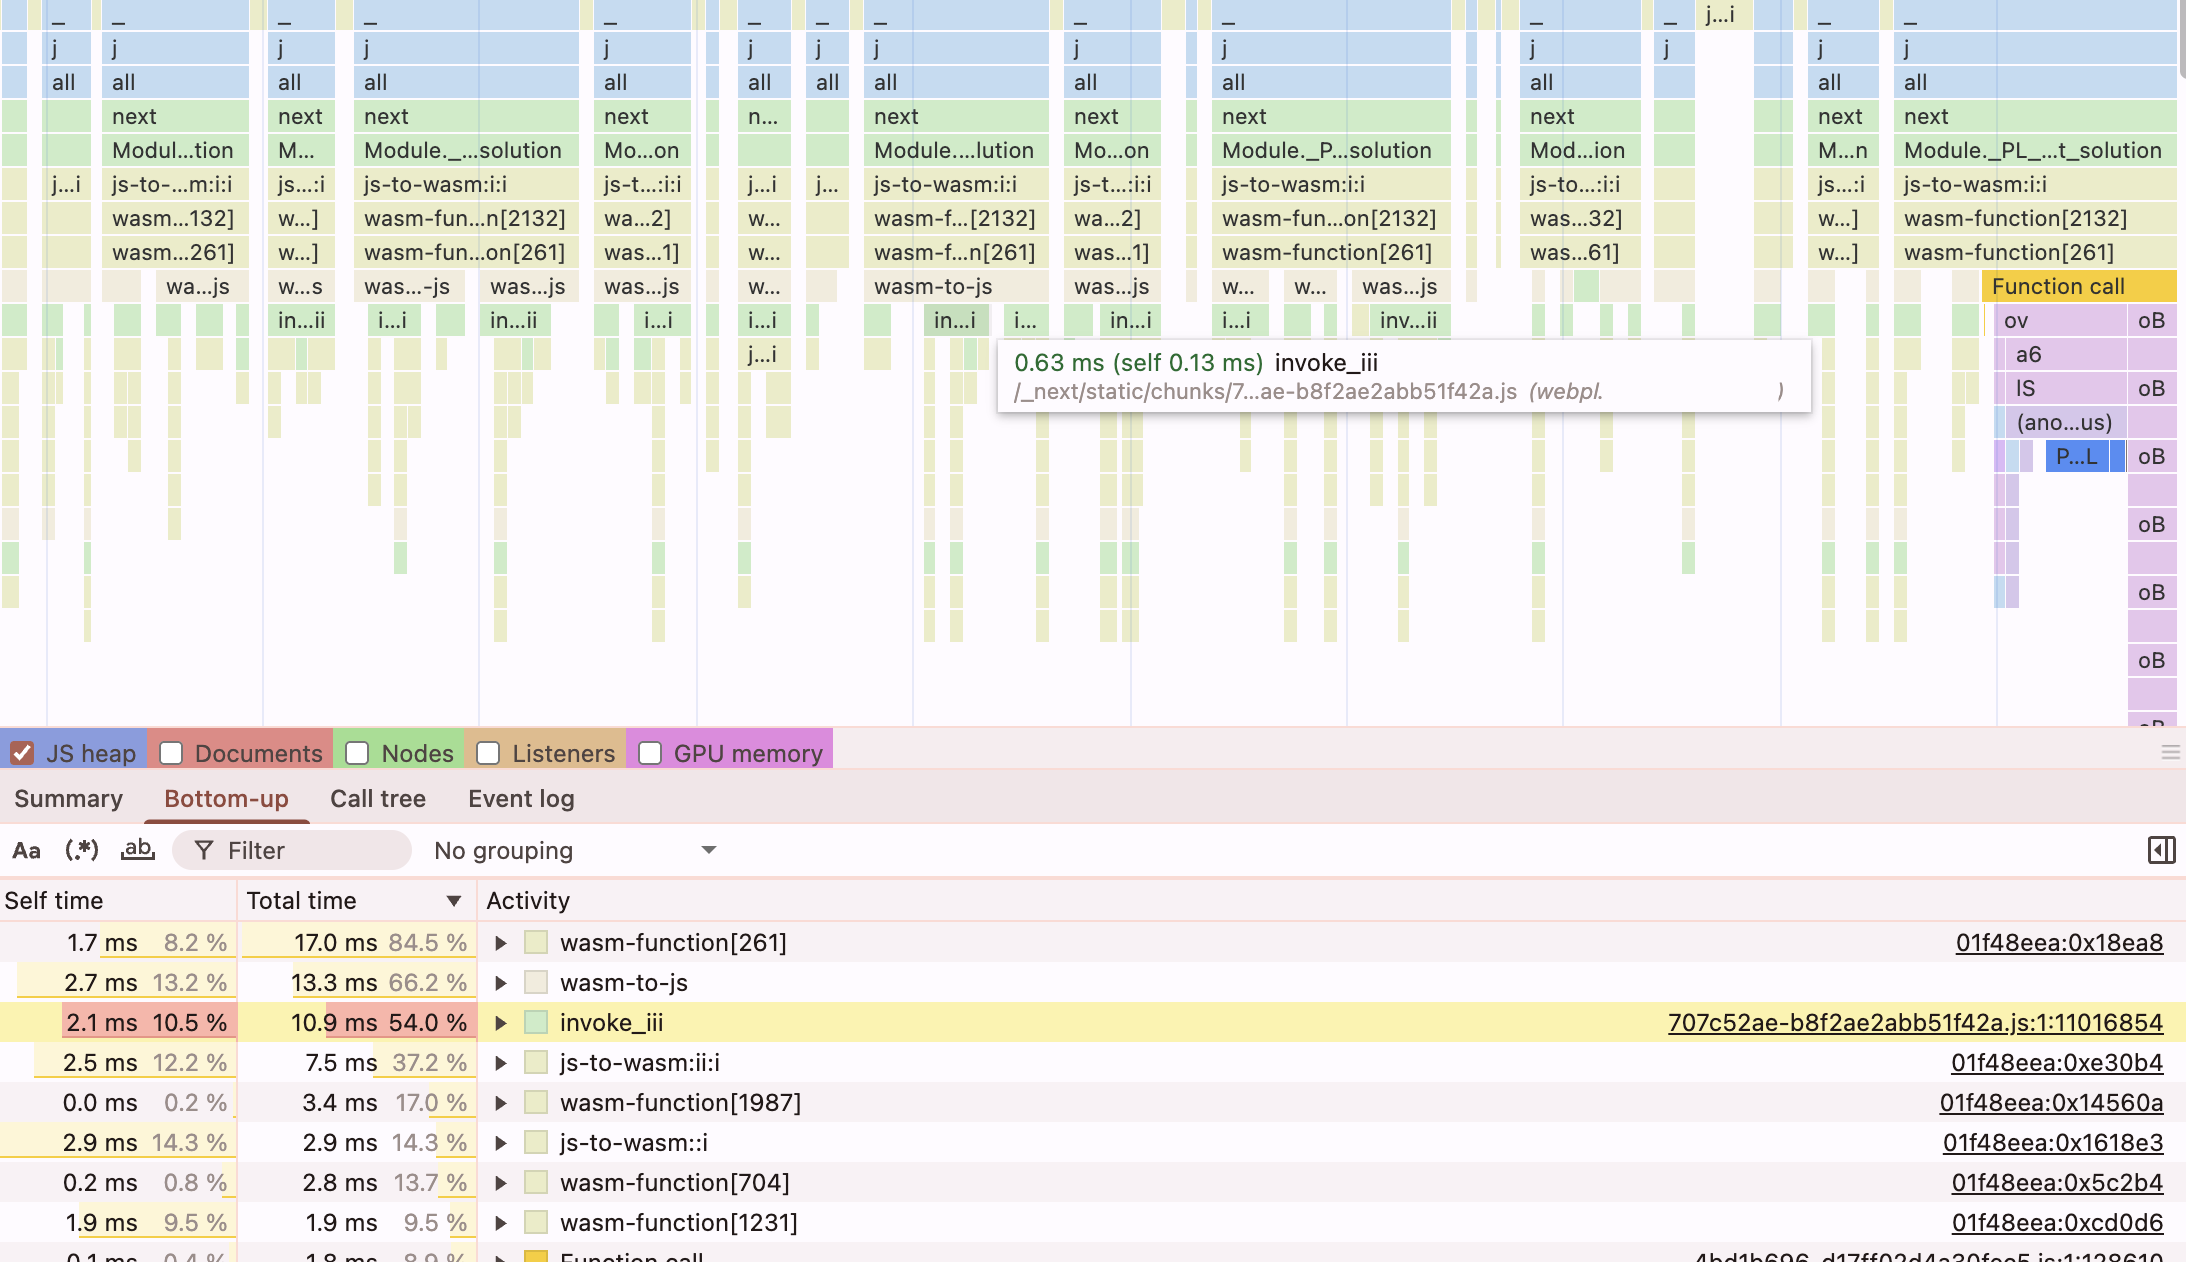
\includegraphics[width=0.8\textwidth]{08evaluation_swiprofiling.png}
\caption{Stack chart of SWI-Prolog execution}
\label{fig:swi-prolog-profile}
\end{figure}

This revealed that a great deal of time is spent crossing the boundary between WebAssembly and JavaScript code, in particular calling the \texttt{invoke\_iii} JavaScript function from WebAssembly, which promptly calls back into WebAssembly. This function is generated by Emscripten, the compiler used to compile SWI-Prolog to WebAssembly, and is shown below.

\begin{center}
\begin{minted}{javascript}
function invoke_iii(A, g, I) {
    var C = stackSave();
    try {
        return getWasmTableEntry(A)(g, I)
    } catch (A) {
        if (stackRestore(C),
        A !== A + 0)
            throw A;
        _setThrew(1, 0)
    }
}
\end{minted}
\end{center}

WebAssembly does not have a built-in exception mechanism, so Emscripten uses JavaScript exceptions instead. \texttt{invoke\_iii} is used to invoke a WebAssembly function that might raise an exception, and perform the necessary stack manipulation to jump back to WebAssembly code that handles the exception if one is raised. This comes at the performance cost of crossing the JavaScript-WebAssembly boundary not only when raising an exception, but also when calling any function that might do so.

SWI-Prolog is written in C, so does not itself use exceptions. However, it supports Prolog exceptions (extra-logical predicates that can be used to implement more complex control flow), and these are implemented using C \texttt{setjmp} and \texttt{longjmp} functions. Emscripten uses the same \texttt{invoke\_iii} mechanism, with its associated cost, to implement these functions.

\subsection{Experimental WebAssembly Exception Support}

While exceptions are not currently supported in WebAssembly, there is a proposal\footnote{\url{https://github.com/WebAssembly/exception-handling/blob/main/proposals/exception-handling/Exceptions.md}} to do so. This has been experimentally implemented in Chrome's V8 JavaScript engine, and can be enabled with the \texttt{--enable-experimental-webassembly-features} flag.

To evaluate the potential performance gains of this feature for SWI-Prolog, I modified the SWI-Prolog build process to enable experimental WebAssembly exception support in Emscripten and Node.js, which is used for some SWI-Prolog tests. SWI-Prolog is built using the Docker container system, so I added the necessary flags in various places in the Dockerfile, as well as making further changes to have it build on the Arm architecture.

\vspace*{-1em}

\begin{verbatim}
-fno-exceptions -s WASM_EXNREF=1 -s SUPPORT_LONGJMP=wasm
\end{verbatim}

\vspace*{-1em}

The benchmark suite was then re-run with the modified SWI-Prolog build in Chrome with experimental WebAssembly exception support enabled. Figure~\ref{fig:swi-prolog-exception} shows the execution time of WebPL and the experimental version of SWI-Prolog, relative to the original version.

\begin{figure}[H]
\centering
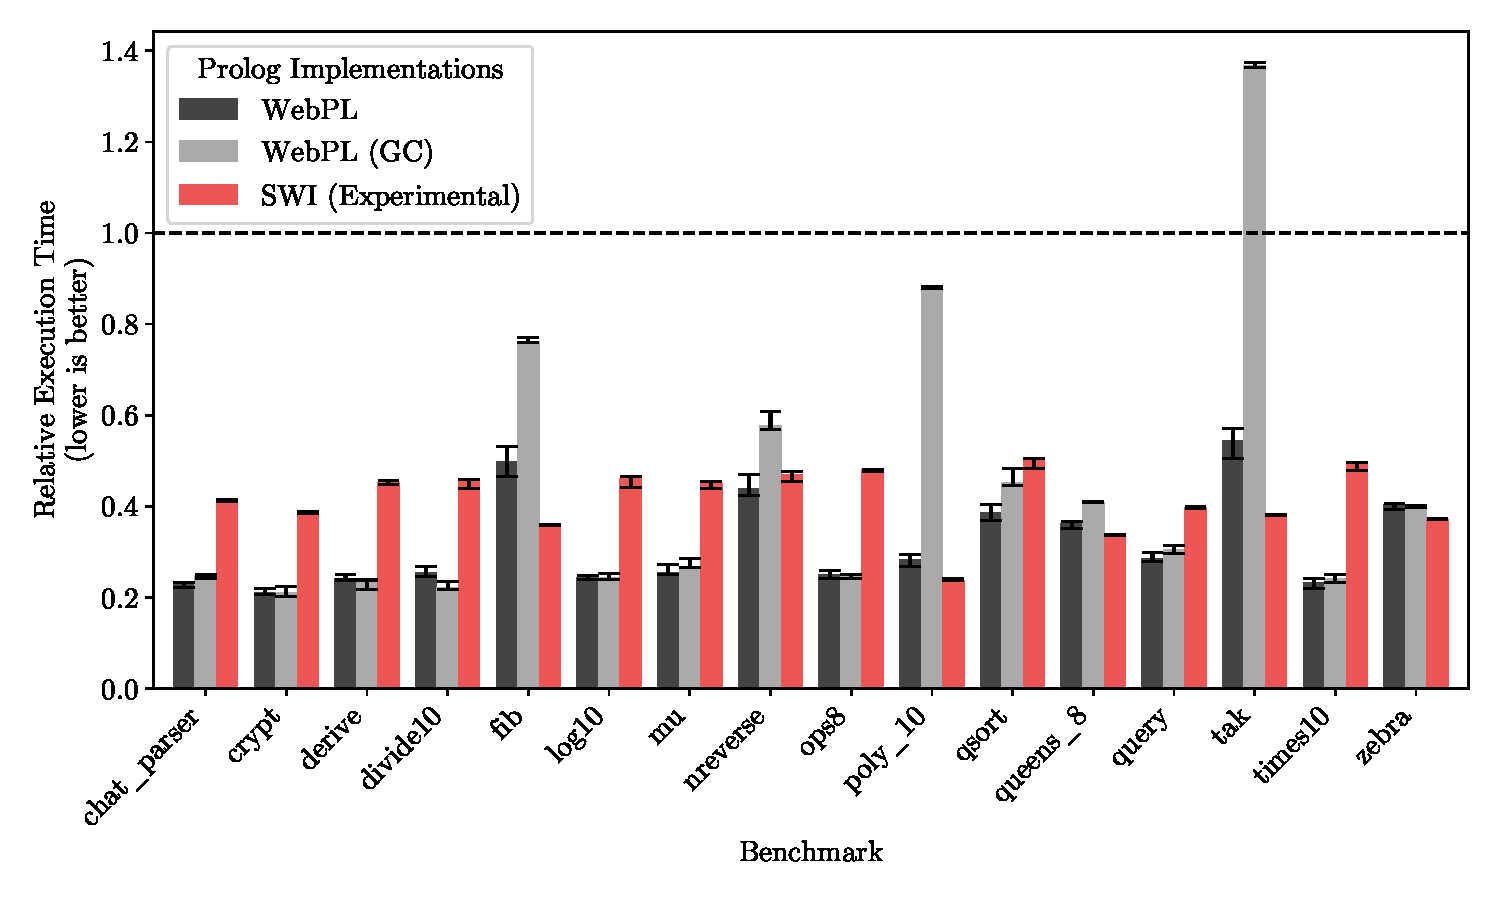
\includegraphics[width=0.8\textwidth]{relative_performance_exnref.pdf}
\caption{Execution time of benchmarks relative to SWI-Prolog}
\label{fig:swi-prolog-exception}
\end{figure}

This shows that enabling experimental WebAssembly exception support in SWI-Prolog reduces execution time by around 60\%, bringing it much closer to, and in some cases surpassing, WebPL.

\subsection{Binary Size}

\label{sec:binary-size-opt}

The size of SWI-Prolog's WebAssembly binary is almost ten times larger than that of WebPL (Section~\ref{sec:binary-size}). It has three distinct parts: the WebAssembly code itself (1.99 MB), libraries (5.80 MB), and JavaScript glue code (0.16 MB). Many of the libraries are not needed in most applications, so I built a ``minimal'' version of SWI-Prolog as a fairer comparison.

The SWI-Prolog build process provides a \texttt{-DSWIPL-PACKAGES=OFF} flag which excludes all libraries except the standard library, reducing the size of the libraries by nearly half to 2.99 MB and the WebAssembly code to 1.23 MB. However, the WebAssembly build depends on the \texttt{clib} library to load Prolog code from a URL. Building with just this library enabled results in WebAssembly code of 1.44 MB and libraries of 3.27 MB.

This is still 0.49 MB more than building without \texttt{clib}. To avoid this 0.49 MB dependency, I rewrote part of the \texttt{wasm.pl} library in the SWI-Prolog source code to use SWI-Prolog's built-in pure-Prolog \texttt{url} library instead of \texttt{clib}, which is partially written in C.

Figure~\ref{fig:binary-size} shows the size of each configuration, and compares them to WebPL.

\begin{figure}[H]
\centering
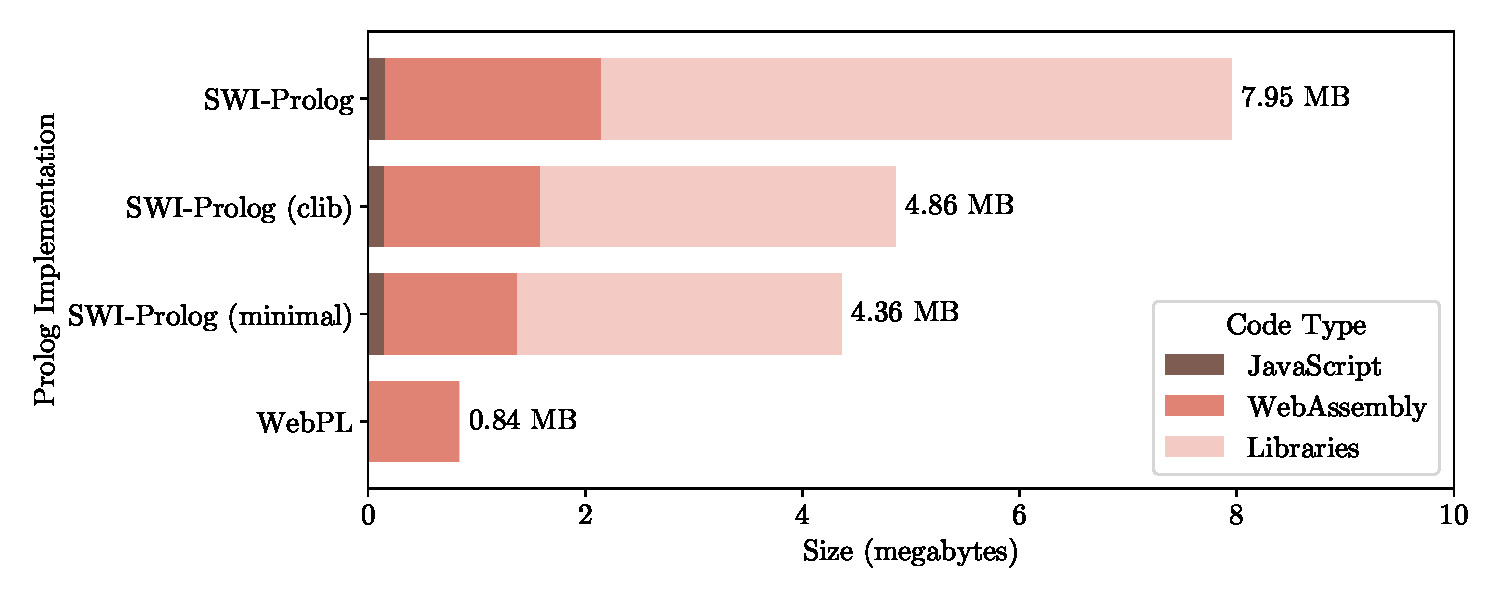
\includegraphics[width=0.8\textwidth]{binary_size.pdf}
\caption{Size of WebAssembly binaries for Prolog implementations}
\label{fig:binary-size}
\end{figure}

\vspace*{-1.5em}

Another approach explored to reduce binary size was the \texttt{wasm-opt} tool, part of the Binaryen project \cite{zakaiBinaryenhttpsgithubcom2015}, configured to optimise aggressively for size using the \texttt{-Oz} flag. However, this only reduced the size of the SWI-Prolog binary by 0.38\%, and WebPL by 0.62\%. This is likely because the compiler is already running code size optimisations by default; indeed, compiling WebPL without optimisations gives a binary size of 14.16 MB, more than 16 times larger than the optimised version.

While WebPL was built from scratch, conscious of its binary size, SWI-Prolog's WebAssembly port was not, and even intentionally avoided some optimisations that would have reduced its binary size in favour of keeping the port closer to the native version\footnote{\url{https://swi-prolog.discourse.group/t/wiki-discussion-swi-prolog-in-the-browser-using-wasm/5651/109}}.

\section{Rust Evaluation}

\label{sec:rust-evaluation}

WebPL is written in Rust to take advantage of its extensive support for WebAssembly and its performance (Section~\ref{sec:tools}). This section explores aspects of Rust that may affect performance.

\subsection{Unsafe Rust}

Rust is known for its memory safety guarantees. Many of these are verified at compile time by the borrow checker, which enforces the ownership and borrowing rules of Rust and prevents common causes of memory errors, such as use-after-free and double-free errors. However, some checks cannot be performed at compile time, such as bounds checking, and are instead performed at runtime, at a performance cost.

Rust provides the \texttt{unsafe} keyword to bypass these checks. This is necessary for interfacing with external code that the borrow checker cannot verify, but can also be used cautiously to improve performance.

WebPL represents the heap as an array of fixed-size terms (Section~\ref{sec:memory-layout}), so indexing into the heap involves a bounds check. By using \texttt{unsafe} to bypass this check, the performance of the Prolog interpreter may improve.

Figure~\ref{fig:unsafe} shows the relative execution time of each benchmark without bounds-checking, compared to the original version of WebPL.

\begin{figure}[H]
\centering
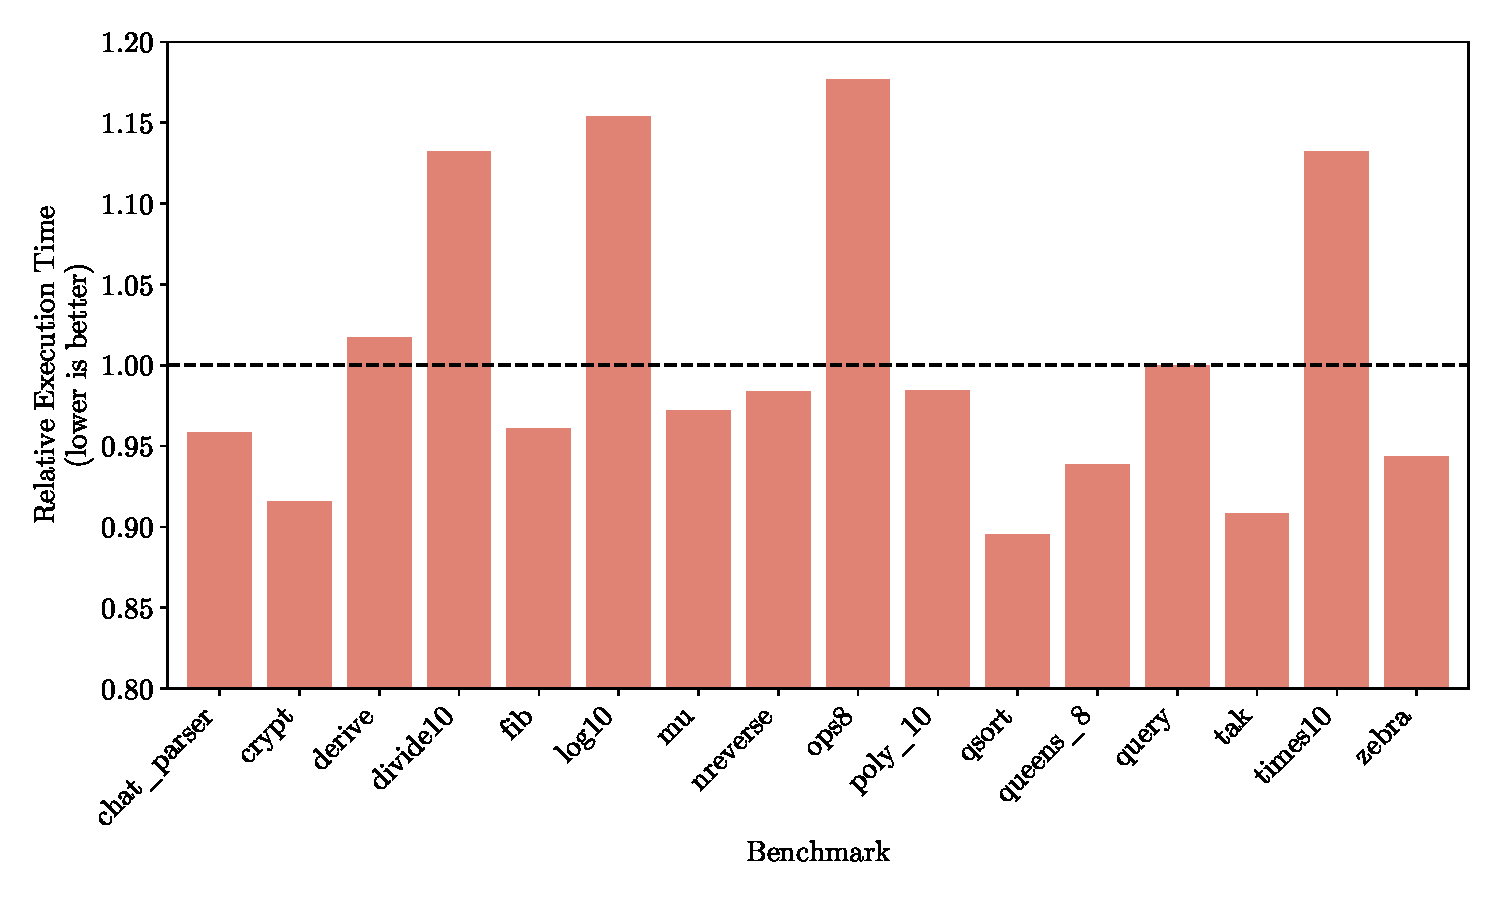
\includegraphics[width=0.8\textwidth]{relative_performance_unsafe.pdf}
\caption{Execution time of unsafe WebPL benchmarks relative to safe WebPL}
\label{fig:unsafe}
\end{figure}

Remarkably, while the more heavyweight benchmarks, like \texttt{fib}, \texttt{queens\_8}, and \texttt{tak}, show an improvement of up to 10\% lower execution time, the lighter benchmarks, like \texttt{divide10}, \texttt{ops8}, and \texttt{times10}, show a degradation of up to 20\% higher execution time. This is likely due to the fact that the overhead of bounds-checking is negligible for lightweight benchmarks, and using unsafe code reduces the compiler's optimisation opportunities.

For this reason, alongside that Rust discourages the use of unsafe code, unsafe code was not used in WebPL.

\subsection{Memory Layout}

Using a Rust \texttt{enum} to represent terms leaves their layout in memory up to the compiler, which may use more memory than necessary to represent them. The exact memory layout in WebAssembly can be inspected using experimental Rust compiler flags:

\begin{verbatim}
$ cargo +nightly rustc --target wasm32-unknown-unknown -- -Zprint-type-sizes
\end{verbatim}

Figure~\ref{fig:memory-layout-wasm} shows the memory layout of an integer atom term and a variable term in WebAssembly. This reveals significant wasted space: flags \texttt{shunted} and \texttt{attributed} use a byte each, and the tag indicating the term type uses 4 bytes, even though one would suffice.

\begin{figure}[H]
\centering
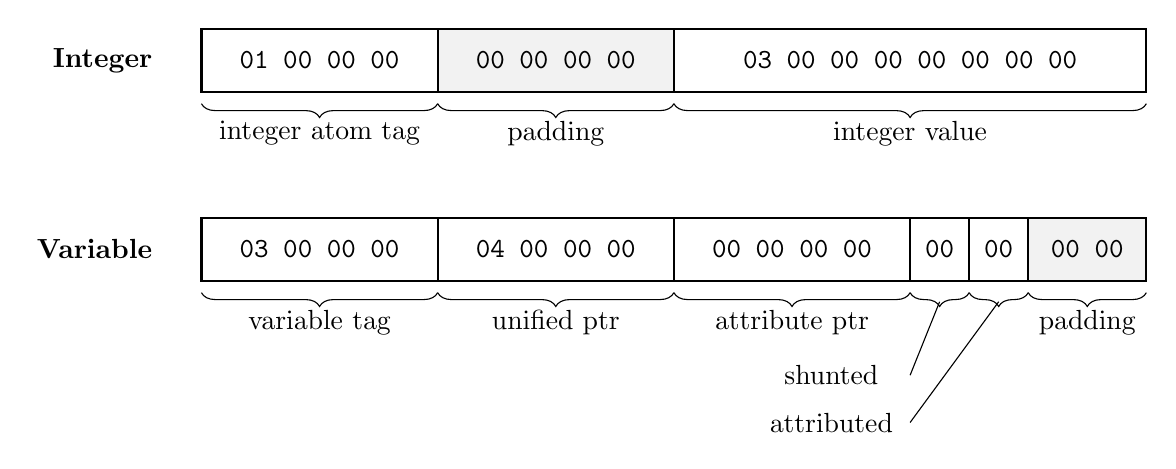
\begin{tikzpicture}[yscale=0.8]

\fill[thick, black!5] (3,0) rectangle (6,1);
\draw[thick] (0,0) rectangle (12,1);

\draw[thick] (3,0) -- (3,1);
\draw[thick] (6,0) -- (6,1);

\node at (1.5,0.5) {\texttt{01 00 00 00}};
\node at (4.5,0.5) {\texttt{00 00 00 00}};
\node at (9,0.5) {\texttt{03 00 00 00 00 00 00 00}};

\draw [decorate,decoration={brace,amplitude=5pt,mirror,raise=1ex}] (0,0) -- (3,0) node[midway,yshift=-1.5em]{integer atom tag};
\draw [decorate,decoration={brace,amplitude=5pt,mirror,raise=1ex}] (3,0) -- (6,0) node[midway,yshift=-1.5em]{padding};
\draw [decorate,decoration={brace,amplitude=5pt,mirror,raise=1ex}] (6,0) -- (12,0) node[midway,yshift=-1.5em]{integer value};

\fill[thick, black!5] (10.5,-3) rectangle (12,-2);
\draw[thick] (0,-3) rectangle (12,-2);

\draw[thick] (3,-3) -- (3,-2);
\draw[thick] (6,-3) -- (6,-2);
\draw[thick] (9,-3) -- (9,-2);
\draw[thick] (9.75,-3) -- (9.75,-2);
\draw[thick] (10.5,-3) -- (10.5,-2);

\node at (1.5,-2.5) {\texttt{03 00 00 00}};
\node at (4.5,-2.5) {\texttt{04 00 00 00}};
\node at (7.5,-2.5) {\texttt{00 00 00 00}};
\node at (9.375,-2.5) {\texttt{00}};
\node at (10.125,-2.5) {\texttt{00}};
\node at (11.25,-2.5) {\texttt{00 00}};

\draw [decorate,decoration={brace,amplitude=5pt,mirror,raise=1ex}] (0,-3) -- (3,-3) node[midway,yshift=-1.5em]{variable tag};
\draw [decorate,decoration={brace,amplitude=5pt,mirror,raise=1ex}] (3,-3) -- (6,-3) node[midway,yshift=-1.5em]{unified ptr};
\draw [decorate,decoration={brace,amplitude=5pt,mirror,raise=1ex}] (6,-3) -- (9,-3) node[midway,yshift=-1.5em]{attribute ptr};
\draw [decorate,decoration={brace,amplitude=5pt,mirror,raise=1ex}] (9,-3) -- (9.75,-3) node[midway,yshift=-1.5em]{};
\draw [decorate,decoration={brace,amplitude=5pt,mirror,raise=1ex}] (9.75,-3) -- (10.5,-3) node[midway,yshift=-1.5em]{};
\draw [decorate,decoration={brace,amplitude=5pt,mirror,raise=1ex}] (10.5,-3) -- (12,-3) node[midway,yshift=-1.5em]{padding};

\node (S) at (8,-4.5) {shunted};
\node (A) at (8,-5.25) {attributed};

\draw (9,-4.5) -- (9.375,-3.333);
\draw (9,-5.25) -- (10.125,-3.333);

\node at (-0.5,0.5) [anchor=east] {\bf Integer};
\node at (-0.5,-2.5) [anchor=east] {\bf Variable};

\end{tikzpicture}
\caption{Memory layout of Prolog terms in WebAssembly}
\label{fig:memory-layout-wasm}
\end{figure}

Padding is used by the compiler to ensure that heap terms are aligned to 8-byte boundaries, which is sensible for performance reasons, and strictly necessary on some architectures. However, this is not the case in WebAssembly, as the WebAssembly specification explicitly states that unaligned accesses must be allowed \cite{rossbergWebAssemblyCoreSpecification2022}, although underlying hardware constraints may mean that they are slower.

Therefore, if a more compact representation of terms were used, consolidating the tag and flags into a single byte and removing padding, the size of each term could be reduced from 16 bytes to 9 bytes, reducing heap usage by 44\%. It is possible that maintaining some alignment would still be a worthwhile trade-off, perhaps 4-byte alignment, but this would require more investigation.

Since Rust does not support this level of control over the memory layout without using unions and unsafe code, a pattern that is far from idiomatic, this is not a change that was easily possible to implement in WebPL. However, if the project were to be rewritten in a language like C++, this could be a worthwhile optimisation to explore.

\chapter{Conclusions}

The project was a success: I built a web-native Prolog implementation using WebAssembly, WebPL, with performance surpassing that of existing Prolog systems, while maintaining tight integration with the browser, thus meeting the success criteria. This demonstrated my original hypothesis (Section~\ref{sec:motivation}) that such a system could be built.

Furthermore, the extension goals of building a browser-based development environment, implementing a precise garbage collector, and developing a JavaScript foreign function interface were also successfully completed, alongside extending the implementation with extra-logical predicates and CLP features, making WebPL a practical and usable Prolog system for the Web.

Benchmarking showed that WebPL outperforms SWI-Prolog, Trealla Prolog, and Tau Prolog in most cases, even when WebAssembly exception handling is enabled in SWI-Prolog to mitigate its performance issues (Section~\ref{sec:swi-prolog-optimisation}). In addition, its memory usage and binary size are both significantly lower than those of other systems, making it suitable for use in resource-constrained environments such as mobile devices.

I have publicly released the project on GitHub under the MIT licence, and I hope that it may be useful to others in the future.

\section{Reflections}

I learnt a huge amount during this project, especially regarding Prolog, garbage collection, and writing a dissertation. Aspects of the project I anticipated to be straightforward turned out to be challenging, in particular correctly implementing the core Prolog interpreter and the garbage collector. This gave rise to several obscure bugs that required me to gain deep understanding of the nuances of Prolog to remedy.

I particularly enjoyed taking the initial prototype of WebPL and iteratively optimising and redesigning it, guided by benchmarking and profiling, to achieve a final result that was 1000x faster than my first working prototype. I am proud to have built a genuinely usable Prolog system that is fast and lightweight.

Were I to do this project again, I would spend more time on the design of the Prolog interpreter to make it more modular and extensible. I found it very challenging to evaluate alternative design decisions after having made the initial choices, and the ability to configure the system at runtime would have made it easier to experiment with different implementations and allow the user to choose the most appropriate one for their use case.

\section{Future Work}

There are several areas I would have explored further, but lacked time to do so. These include:

\begin{itemize}
\item \emph{JIT compilation}: The current implementation of WebPL is an interpreter, with limited pre-execution static analysis to optimise the execution of Prolog code. A just-in-time (JIT) compiler could be implemented to compile Prolog code either to the instruction set of a virtual machine, such as the WAM, or directly to WebAssembly. There are several key questions for such an implementation to address, including how to maintain WebPL's tight integration with the browser and with JavaScript from compiled code.
\item \emph{ISO compliance}: Compliance with the ISO Prolog standard \cite{isoInformationtechnologyProgramming1995} is a goal of many Prolog implementations, and one that cements an implementation's credibility. WebPL is not yet fully compliant with the ISO standard, instead implementing a subset of the standard that is sufficient for this dissertation, but full ISO compliance would be a worthy goal for future work.
\item \emph{C++ implementation}: Many limitations of WebPL arise from the Rust programming language (Section~\ref{sec:rust-evaluation}). Reimplementing the project in C++ may provide more opportunities for optimisation, and more flexibility and control over the exact behaviour of the system. While C++ does not make the strong memory safety guarantees of Rust, WebAssembly prevents memory safety bugs from causing security vulnerabilities.
\end{itemize}

\addcontentsline{toc}{chapter}{Bibliography}
\bibliographystyle{apalike}
\bibliography{refs}

\begin{appendices}

\chapter{JavaScript-WebAssembly Interaction}

\label{appendix:shared-memory}

To illustrate the interaction described in \ref{sec:wasm-js-interface}, consider the example in Figure \ref{fig:js-wasm} where JavaScript passes a value to WebAssembly through the linear memory, and WebAssembly calls back into JavaScript to output that value. The JavaScript \texttt{DataView} API is used to write an integer value to the linear memory, specifying little-endian byte order, and the WebAssembly function \texttt{get} loads the value and calls the imported JavaScript function \texttt{log} to output it.

\begin{figure}[H]
\centering
\begin{subfigure}{\textwidth}
\begin{minted}{javascript}
/* Instantiate the WebAssembly module, providing `console.log` as an external
 * function to call from within WebAssembly. */
WebAssembly.instantiate(fetch("a.wasm"), { env: { log: console.log } })
  .then(({ instance }) => {
    /* Use the built-in DataView API to write a value of a specific size and
     * endianness to the linear memory, in this case writing the integer 1234
     * as a 32-bit little-endian signed integer to address 0. */
    const mem = new DataView(instance.exports.memory.buffer);
    mem.setInt32(0, 1234, /*littleEndian=*/true);

    /* Call the WebAssembly function `get`, passing the address of the value
     * that was just written to the linear memory. */
    instance.exports.get(0);
  });
\end{minted}
\caption{JavaScript code to write to linear memory and call into WebAssembly}
\end{subfigure}
\par\bigskip
\par\bigskip
\begin{subfigure}{\textwidth}
\begin{minted}{asm}
(module
  ;; Import external function `log` specified when instantiating the module.
  (import "env" "log" (func $log (param i32)))

  ;; Make the linear memory accessible from JavaScript.
  (memory (export "memory") 1)

  (func (export "get") (param $ptr i32)
    local.get $ptr ;; push the pointer onto the stack
    i32.load       ;; load the value from linear memory
    call $log      ;; pass the value to the JavaScript function
  )
)
\end{minted}
\caption{WebAssembly code to read from linear memory and call into JavaScript}
\end{subfigure}
\caption{JavaScript-WebAssembly interaction}
\label{fig:js-wasm}
\end{figure}

\chapter{Built-in Predicates}

\label{appendix:predicates}

\section{Predicates}

Supported built-in predicates (Section \ref{sec:builtins}) are shown in Table \ref{table:predicates}.

\begin{table}
\centering
\begin{tabular}{lp{12cm}}
\hline
\textbf{Predicate} & \textbf{Description} \\
\hline
\texttt{is/2} & Unifies the first argument with the result of evaluating the second argument, or fails if they do not unify. \\
\texttt{=/2} & Unifies the first argument with the second argument, or fails if they do not unify. \\
\texttt{>/2} & Succeeds if the first argument is greater than the second argument. \\
\texttt{</2} & Succeeds if the first argument is less than the second argument. \\
\texttt{>=/2} & Succeeds if the first argument is greater than or equal to the second argument. \\
\texttt{=</2} & Succeeds if the first argument is less than or equal to the second argument. \\
\texttt{=\textbackslash=/2} & Succeeds if the first argument is not equal (arithmetic) to the second argument. \\
\texttt{=:=/2} & Succeeds if the first argument is equal (arithmetic) to the second argument. \\
\texttt{==/2} & Succeeds if the first argument is equal (term) to the second argument. \\
\texttt{delay/2} & Delays the evaluation of the second argument until the first is bound (see Section \ref{sec:attributed-variables}). \\
\texttt{freeze/2} & Delays the evaluation of the second argument until the first is bound to a non-variable (see Section \ref{sec:attributed-variables}). \\
\texttt{integer/1} & Succeeds if the argument is an integer. \\
\texttt{float/1} & Succeeds if the argument is a floating point number. \\
\texttt{atom/1} & Succeeds if the argument is an atom. \\
\texttt{var/1} & Succeeds if the argument is a variable. \\
\texttt{nonvar/1} & Succeeds if the argument is not a variable. \\
\texttt{compound/1} & Succeeds if the argument is a compound term. \\
\texttt{number/1} & Succeeds if the argument is a number (integer or float). \\
\texttt{!/0} & Cut operator. \\
\texttt{statistics/2} & Queries runtime statistics, see Table \ref{table:statistics}. \\
\hline
\end{tabular}
\caption{Built-in predicates}
\label{table:predicates}
\end{table}

\section{Statistics Predicate}

The \texttt{statistics/2} predicate takes a statistic name as its first argument, unifying the current value of that statistic with the second argument. Available statistics are shown in Table \ref{table:statistics}.

\begin{table}
\centering
\begin{tabular}{ll}
\hline
\textbf{Statistic} & \textbf{Description} \\
\hline
\texttt{memory} & Current heap memory usage in bytes. \\
\texttt{allocated} & Current allocated heap size in bytes. \\
\texttt{gc} & Number of garbage collections performed. \\
\texttt{wasm\_memory} & Current size of the WebAssembly linear memory in bytes. \\
\hline
\end{tabular}
\caption{Supported statistics}
\label{table:statistics}
\end{table}

\chapter{JavaScript FFI Built-In Functions}

\label{appendix:js-ffi}

\begin{table}[H]
\centering
\begin{tabular}{lp{12cm}}
\hline
\textbf{Function} & \textbf{Description} \\
\hline
\texttt{unify} & Performs unification. Both terms must be valid JavaScript representations of Prolog terms (Section \ref{sec:js-prolog-mapping}), which will be converted back to Prolog terms and allocated on the heap if necessary. Variable bindings are checked to ensure they refer to terms that exist. \\
\texttt{fetch} & Makes a synchronous HTTP request to the given URL, returning the response as a string. This is implemented in JavaScript as a wrapper around \texttt{XMLHttpRequest}, provided for convenience. \\
\texttt{compound} & Creates a compound term from a functor and some arguments. \\
\texttt{list} & Converts a JavaScript list into its linked-list Prolog representation. \\
\hline
\end{tabular}
\caption{Functions available to JavaScript code}
\label{tab:js-ffi}
\end{table}

\chapter{Benchmark Programs}

\label{appendix:benchmarks}

\begin{table}[H]
\centering
\begin{tabular}{ll}
\hline
\textbf{Benchmark} & \textbf{Description} \\
\hline
chat\_parser & Parse natural language \\
crypt & Cryptomultiplication \\
derive & Symbolic differentiation \\
divide10 & Symbolic differentiation \\
fib & Fibonacci sequence \\
log10 & Symbolic differentiation \\
mu & MU puzzle \\
nreverse & Naive list reversal \\
ops8 & Symbolic differentiation \\
poly\_10 & Polynomial exponentiation \\
qsort & Quicksort \\
queens\_8 & 8-Queens problem \\
query & Query deductive database \\
tak & Takeuchi function \\
times10 & Symbolic differentiation \\
zebra & Zebra puzzle \\
\hline
\end{tabular}
\caption{Selected benchmarks from the SWI-Prolog benchmark suite}
\label{tab:benchmarks}
\end{table}

\chapter{Project Proposal}

\label{appendix:proposal}

\includepdf[pages=-]{../proposal/proposal.pdf}

\end{appendices}

\end{document}